% ==========================================
% CASOS DE USO Y DIAGRAMAS EXTRA (CU4 - CU12)
% ==========================================

En este apéndice se amplía el contenido presentado en la \autoref{SEC:AD_CASOSUSO}, detallando el resto de casos de uso secundarios de la aplicación junto con sus respectivos diagramas de secuencia. Dichos casos de uso son: registro de usuario (\autoref{TB:CU4_REGISTRO} y \autoref{FIG:CU4_SEQ}), inicio de sesión (\autoref{TB:CU5_LOGIN} y \autoref{FIG:CU5_SEQ}), cierre de sesión (\autoref{TB:CU6_LOGOUT} y \autoref{FIG:CU6_SEQ}), modificación de datos del perfil (\autoref{TB:CU7_PERFIL_DATOS} y \autoref{FIG:CU7_SEQ}), cambio de contraseña (\autoref{TB:CU8_PERFIL_PASSWORD} y \autoref{FIG:CU8_SEQ}), recuperación de contraseña olvidada (\autoref{TB:CU9_RECUPERAR_PASSWORD} y \autoref{FIG:CU9_SEQ}), renombrado manual de sesión de chat (\autoref{TB:CU10_RENOMBRAR_SESION} y \autoref{FIG:CU10_SEQ}), eliminación permanente de sesión de chat (\autoref{TB:CU11_ELIMINAR_SESION} y \autoref{FIG:CU11_SEQ}) y consulta del historial de sesiones (\autoref{TB:CU12_HISTORIAL} y \autoref{FIG:CU12_SEQ}).

\vspace{0.5cm}

\begingroup
\shorthandoff{"<>"}
\setlength{\arrayrulewidth}{1pt}
\arrayrulecolor{vlepsbased}
\begin{longtable}{|p{15cm}|}
  \hline
  \rowcolor{maincolor} 
  \multicolumn{1}{|l|}{\textcolor{white}{\textbf{Caso de Uso}}} \\
  \hline
  \endfirsthead
  \multicolumn{1}{c}{{\tablename\ \thetable{} -- Continuación}} \\
  \hline
  \rowcolor{maincolor} 
  \multicolumn{1}{|l|}{\textcolor{white}{\textbf{Caso de Uso (Continuación)}}} \\
  \hline
  \endhead
  \hline \multicolumn{1}{|r|}{\textit{Continúa en la siguiente página...}} \\ \hline
  \endfoot
  \hline
  \caption{Caso de Uso CU4 — Registro de usuario en la plataforma.}
  \label{TB:CU4_REGISTRO}
  \endlastfoot

  \rowcolor{ulepsbased}
  \begin{tabularx}{\linewidth}{@{}X X@{}}
    \textbf{Identificador:} CU4 & \textbf{Actor principal:} Usuario no autenticado
  \end{tabularx} \\ \hline

  \textbf{Nombre:} Registro de usuario en la plataforma \\ \hline

  \rowcolor{ulepsbased}
  \textbf{Descripción:} \newline 
  El sistema permite a un nuevo usuario crear una cuenta proporcionando nombre de usuario, correo electrónico y contraseña. El sistema verifica que la contraseña sea segura y cifra las credenciales. \\ \hline

  \textbf{Precondiciones:} \newline
  1. El usuario no ha iniciado sesión. \newline
  2. El correo electrónico introducido no está en uso en el sistema. \\ \hline

  \rowcolor{ulepsbased}
  \textbf{Flujo principal:} \newline
  1. El usuario accede a la vista de registro. \newline
  2. Introduce nombre de usuario, email, y repite dos veces una contraseña segura. \newline
  3. Pulsa el botón "Registrarse". \newline
  4. El sistema valida el formato del email y la seguridad de la contraseña (longitud mínima, caracteres alfanuméricos). \newline
  5. El sistema verifica que el nombre de usuario y el email no estén duplicados en la base de datos. \newline
  6. El sistema crea el usuario, realizando un hash seguro de la contraseña (PBKDF2 con SHA-256). \newline
  7. El sistema confirma el registro y redirige automáticamente al usuario a la vista de inicio de sesión. \\ \hline

  \textbf{Flujos alternativos:} \newline
  \textbf{FA-01:} La contraseña es débil o no coincide: \newline
  1. El sistema detecta que las contraseñas no coinciden o no cumplen la política de seguridad. \newline
  2. Se aborta la creación del usuario. \newline
  3. El sistema muestra un mensaje de error específico y devuelve al usuario al formulario. \newline
  \textbf{FA-02:} El usuario o email ya existen: \newline
  1. El sistema detecta que las credenciales pertenecen a otra cuenta. \newline
  2. Se rechaza el registro y se informa al usuario. \\ \hline

  \rowcolor{ulepsbased}
  \textbf{Postcondiciones:} \newline
  1. Se genera un nuevo registro en la base de datos de usuarios. \newline
  2. El usuario está listo para iniciar sesión. \\ \hline

\end{longtable}
\endgroup

\begin{figure}[Diagrama de secuencia CU4]{FIG:CU4_SEQ}{Diagrama de secuencia del registro.}
    \centering
    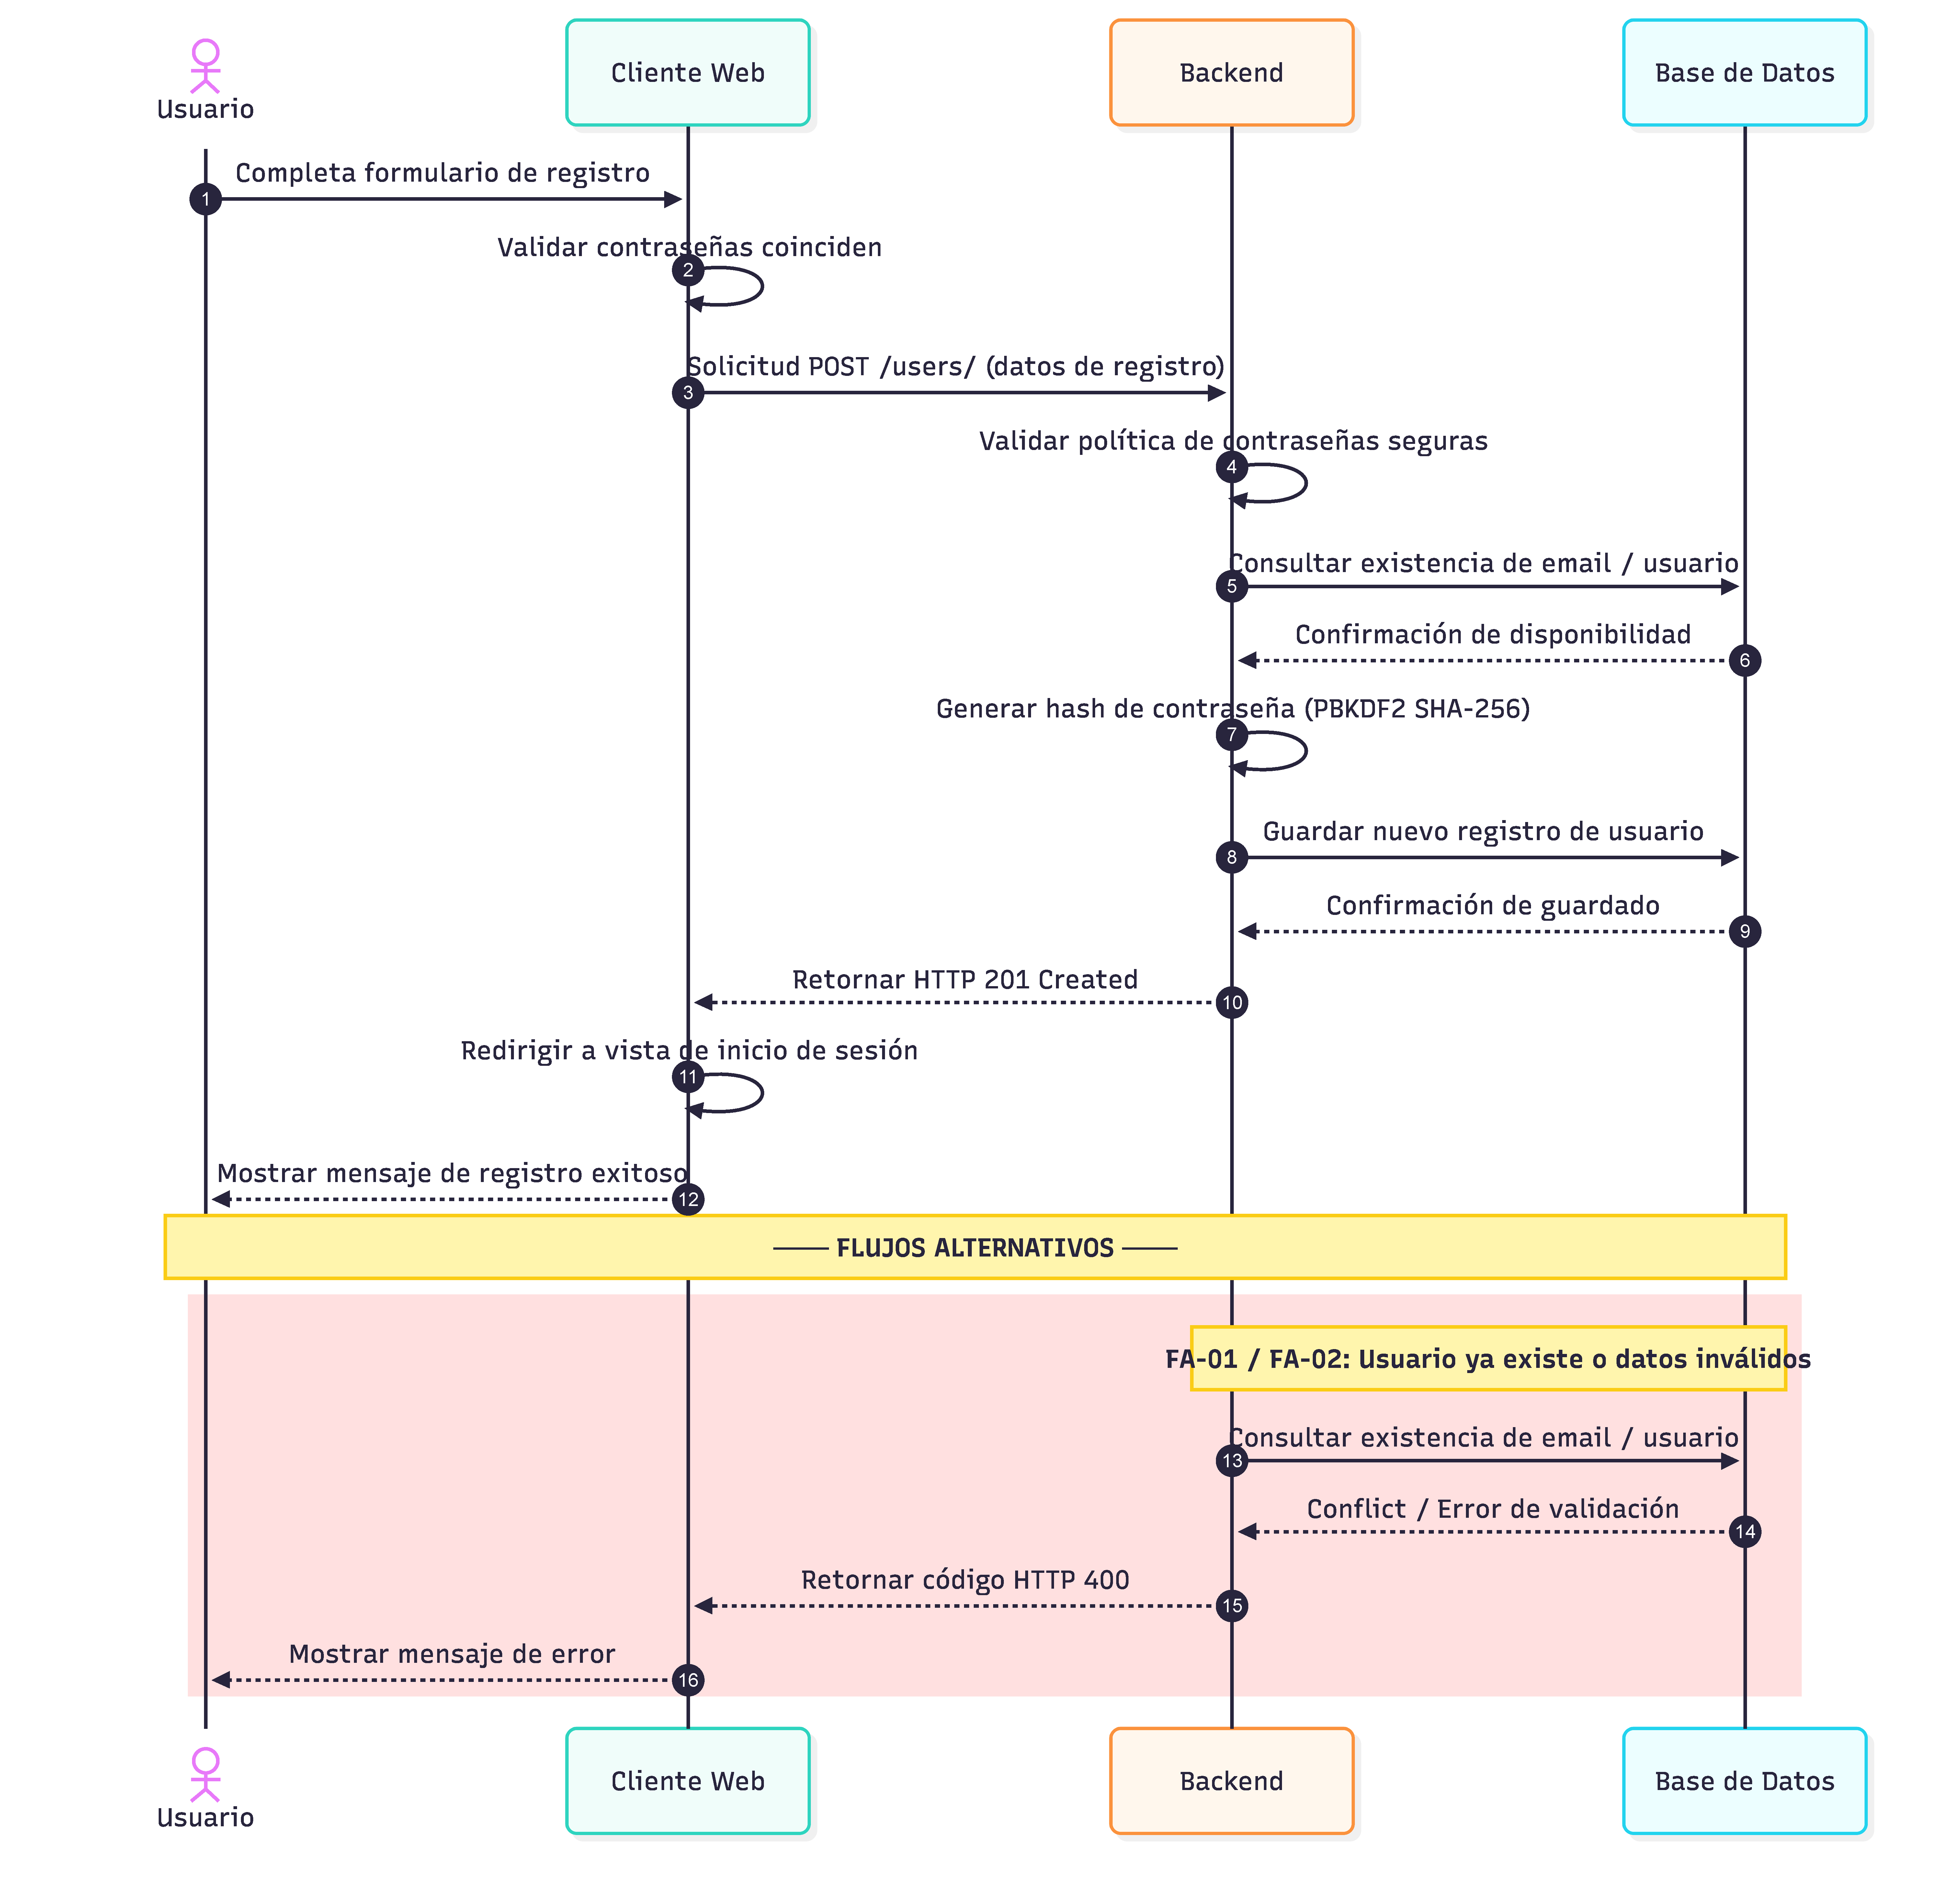
\includegraphics[width=0.85\textwidth]{./diagramas/secuencia_registro_SIMPLE.pdf}
\end{figure}

\begingroup
\shorthandoff{"<>"}
\setlength{\arrayrulewidth}{1pt}
\arrayrulecolor{vlepsbased}
\begin{longtable}{|p{15cm}|}
  \hline
  \rowcolor{maincolor} 
  \multicolumn{1}{|l|}{\textcolor{white}{\textbf{Caso de Uso}}} \\
  \hline
  \endfirsthead
  \multicolumn{1}{c}{{\tablename\ \thetable{} -- Continuación}} \\
  \hline
  \rowcolor{maincolor} 
  \multicolumn{1}{|l|}{\textcolor{white}{\textbf{Caso de Uso (Continuación)}}} \\
  \hline
  \endhead
  \hline \multicolumn{1}{|r|}{\textit{Continúa en la siguiente página...}} \\ \hline
  \endfoot
  \hline
  \caption{Caso de Uso CU5 — Inicio de sesión en la plataforma.}
  \label{TB:CU5_LOGIN}
  \endlastfoot

  \rowcolor{ulepsbased}
  \begin{tabularx}{\linewidth}{@{}X X@{}}
    \textbf{Identificador:} CU5 & \textbf{Actor principal:} Usuario
  \end{tabularx} \\ \hline

  \textbf{Nombre:} Inicio de sesión en la plataforma \\ \hline

  \rowcolor{ulepsbased}
  \textbf{Descripción:} \newline 
  El usuario se autentica en la plataforma mediante sus credenciales. \\ \hline

  \textbf{Precondiciones:} \newline
  1. El usuario debe existir en el sistema. \\ \hline

  \rowcolor{ulepsbased}
  \textbf{Flujo principal:} \newline
  1. El usuario accede a la vista de "Inicio de sesión". \newline
  2. Introduce su usuario y su contraseña. \newline
  3. Pulsa "Ingresar". \newline
  4. El sistema valida las credenciales verificando el hash almacenado. \newline
  5. El sistema genera los tokens JWT de acceso y refresco correspondientes. \newline
  6. El sistema devuelve los tokens y redirige al panel principal del tutor. \\ \hline

  \textbf{Flujos alternativos:} \newline
  \textbf{FA-01:} Credenciales incorrectas: \newline
  1. El sistema detecta que el usuario no existe o la contraseña no es válida. \newline
  2. Se deniega el acceso, no se generan los tokens y se muestra un error al usuario. \\ \hline

  \rowcolor{ulepsbased}
  \textbf{Postcondiciones:} \newline
  1. El usuario tiene acceso a la plataforma. \\ \hline

\end{longtable}
\endgroup

\begin{figure}[Diagrama de secuencia CU5]{FIG:CU5_SEQ}{Diagrama de secuencia del login.}
    \centering
    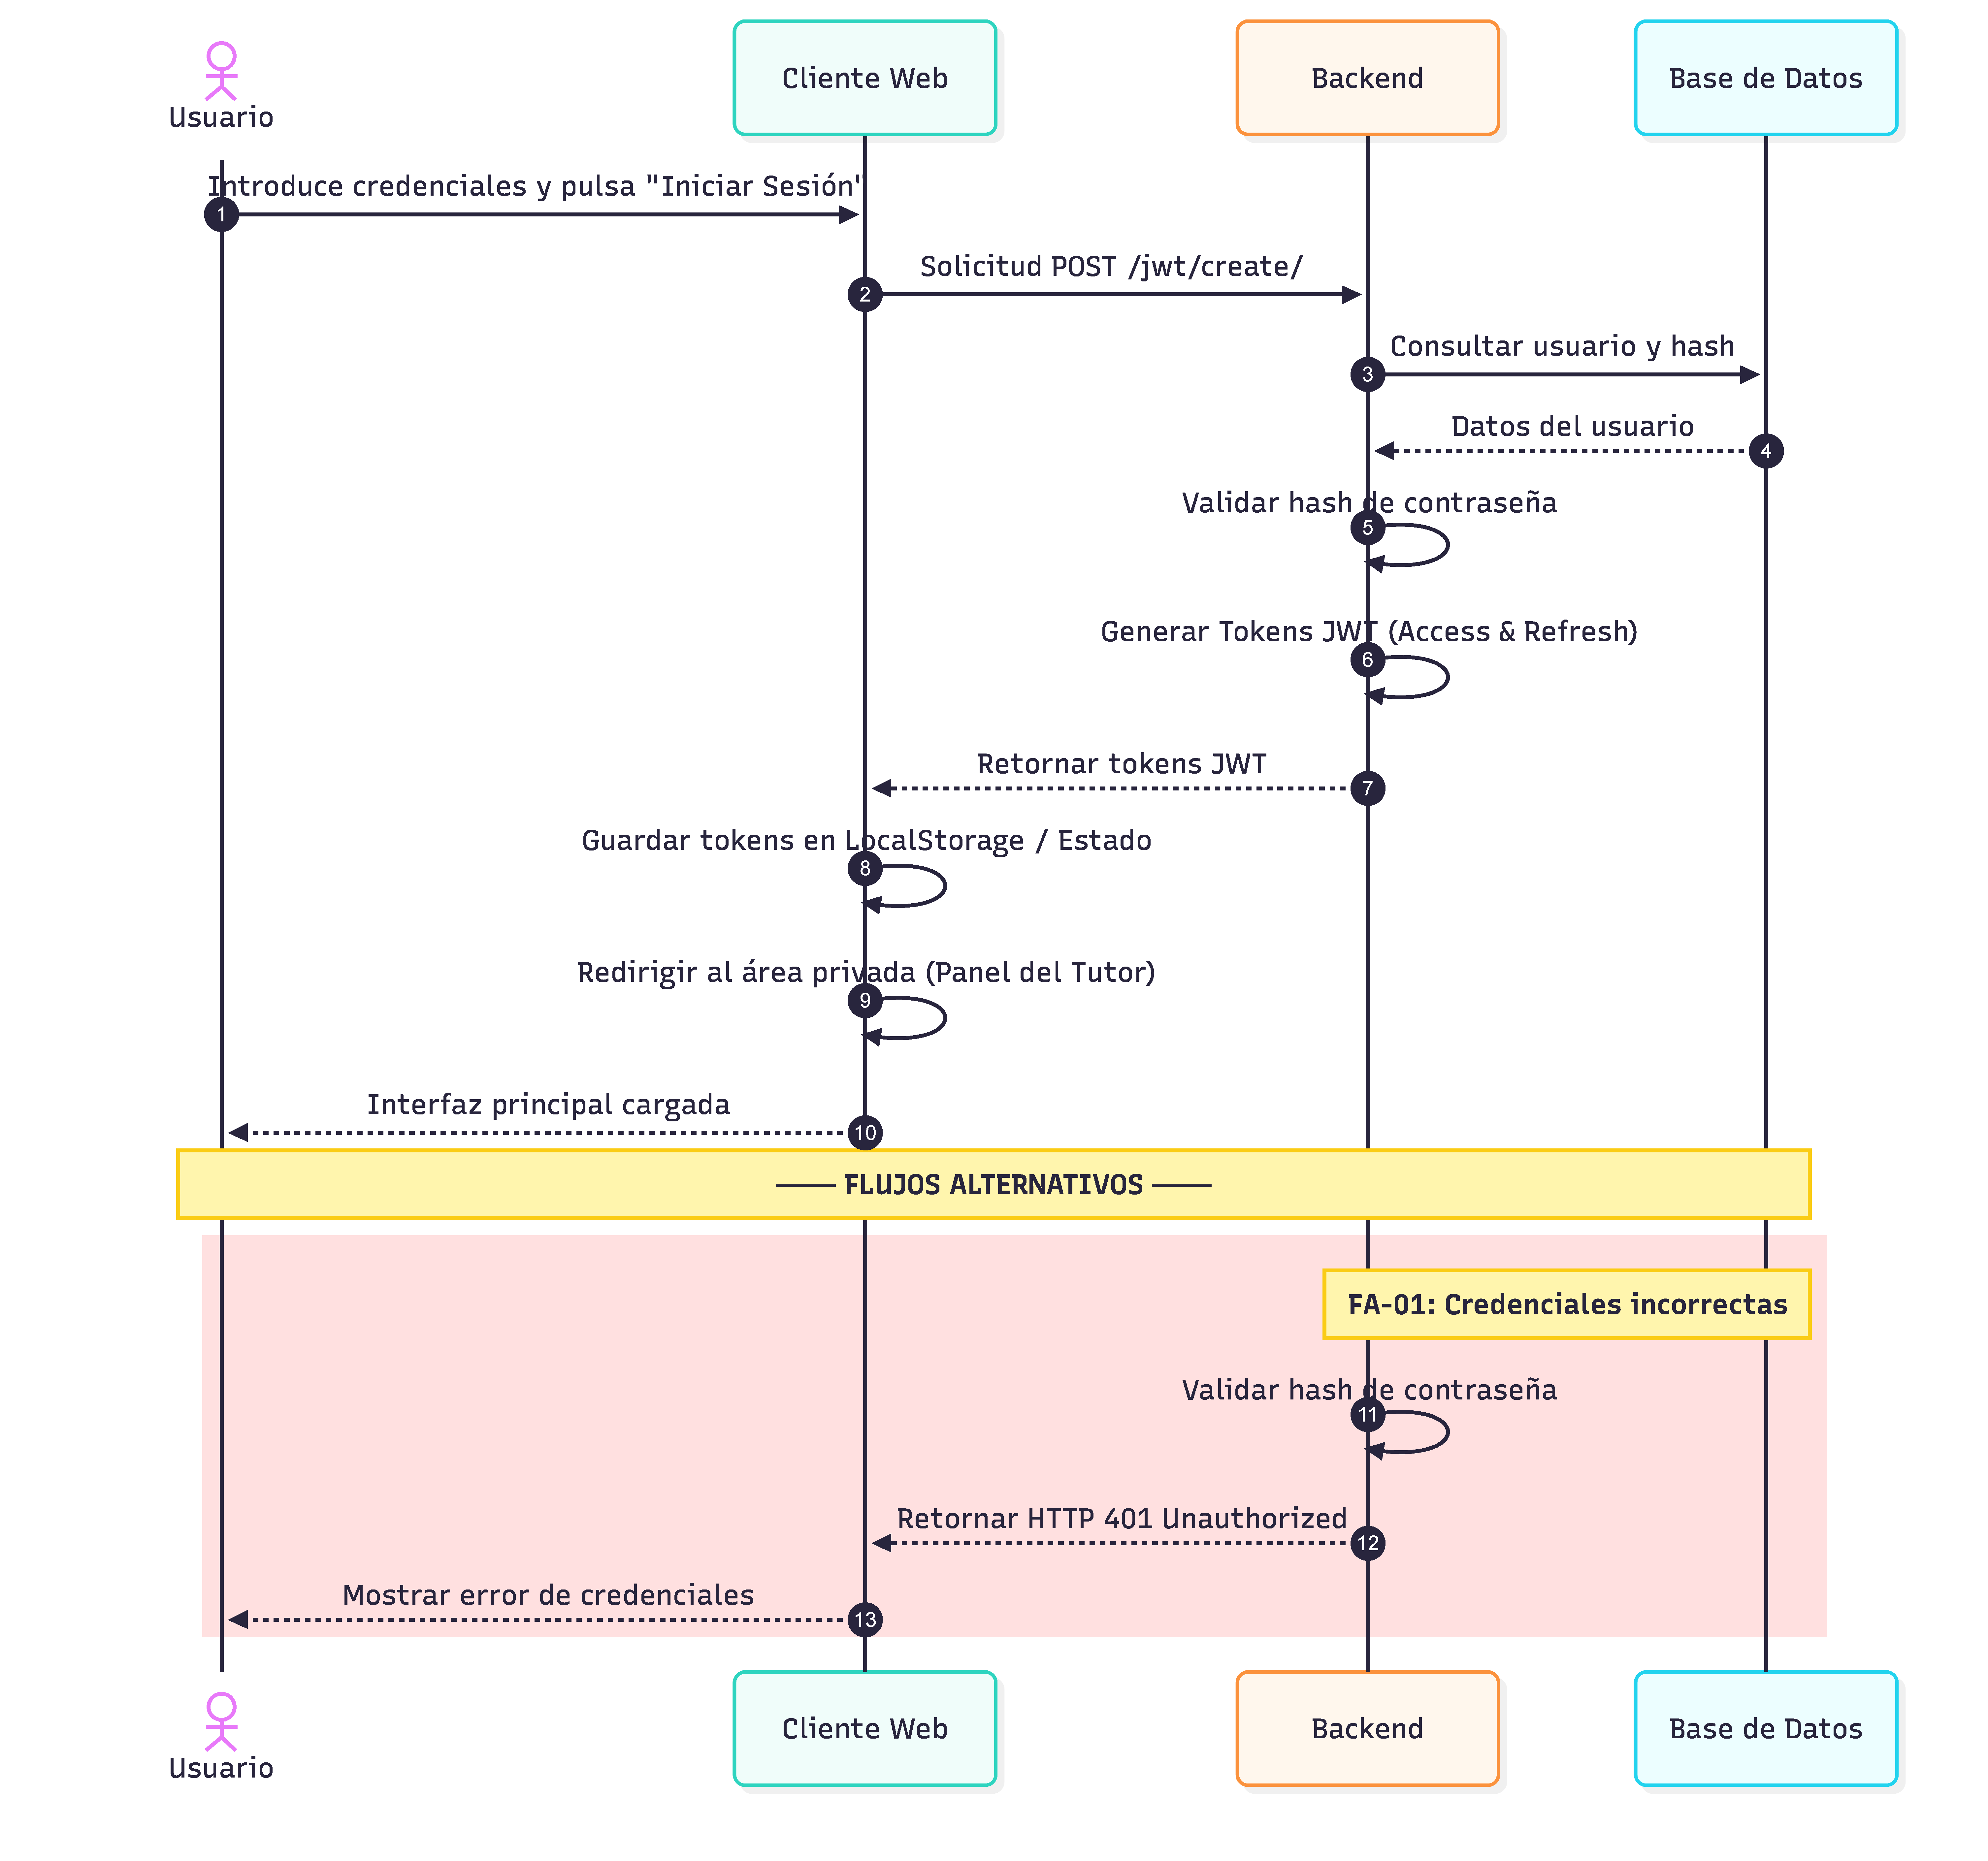
\includegraphics[width=0.85\textwidth]{./diagramas/secuencia_login_SIMPLE.pdf}
\end{figure}

\begingroup
\shorthandoff{"<>"}
\setlength{\arrayrulewidth}{1pt}
\arrayrulecolor{vlepsbased}
\begin{longtable}{|p{15cm}|}
  \hline
  \rowcolor{maincolor} 
  \multicolumn{1}{|l|}{\textcolor{white}{\textbf{Caso de Uso}}} \\
  \hline
  \endfirsthead
  \multicolumn{1}{c}{{\tablename\ \thetable{} -- Continuación}} \\
  \hline
  \rowcolor{maincolor} 
  \multicolumn{1}{|l|}{\textcolor{white}{\textbf{Caso de Uso (Continuación)}}} \\
  \hline
  \endhead
  \hline \multicolumn{1}{|r|}{\textit{Continúa en la siguiente página...}} \\ \hline
  \endfoot
  \hline
  \caption{Caso de Uso CU6 — Cierre de sesión.}
  \label{TB:CU6_LOGOUT}
  \endlastfoot

  \rowcolor{ulepsbased}
  \begin{tabularx}{\linewidth}{@{}X X@{}}
    \textbf{Identificador:} CU6 & \textbf{Actor principal:} Usuario
  \end{tabularx} \\ \hline

  \textbf{Nombre:} Cierre de sesión \\ \hline

  \rowcolor{ulepsbased}
  \textbf{Descripción:} \newline 
  El usuario finaliza su actividad y cierra su sesión de forma segura revocando sus tokens de acceso. \\ \hline

  \textbf{Precondiciones:} \newline
  1. El usuario debe tener una sesión activa iniciada. \\ \hline

  \rowcolor{ulepsbased}
  \textbf{Flujo principal:} \newline
  1. El usuario autenticado pulsa "Cerrar sesión" en el menú de opciones. \newline
  2. El sistema solicita la invalidación del token de refresco en el servidor (blacklist). \newline
  3. El cliente borra los tokens del almacenamiento local. \newline
  4. El usuario es redirigido a la vista de inicio de sesión. \\ \hline

  \textbf{Flujos alternativos:} \newline
  Ninguno. \\ \hline

  \rowcolor{ulepsbased}
  \textbf{Postcondiciones:} \newline
  1. Se destruye el contexto de sesión segura. \newline
  2. El usuario pierde el acceso a las áreas privadas. \\ \hline

\end{longtable}
\endgroup

\begin{figure}[Diagrama de secuencia CU6]{FIG:CU6_SEQ}{Diagrama de secuencia del logout.}
    \centering
    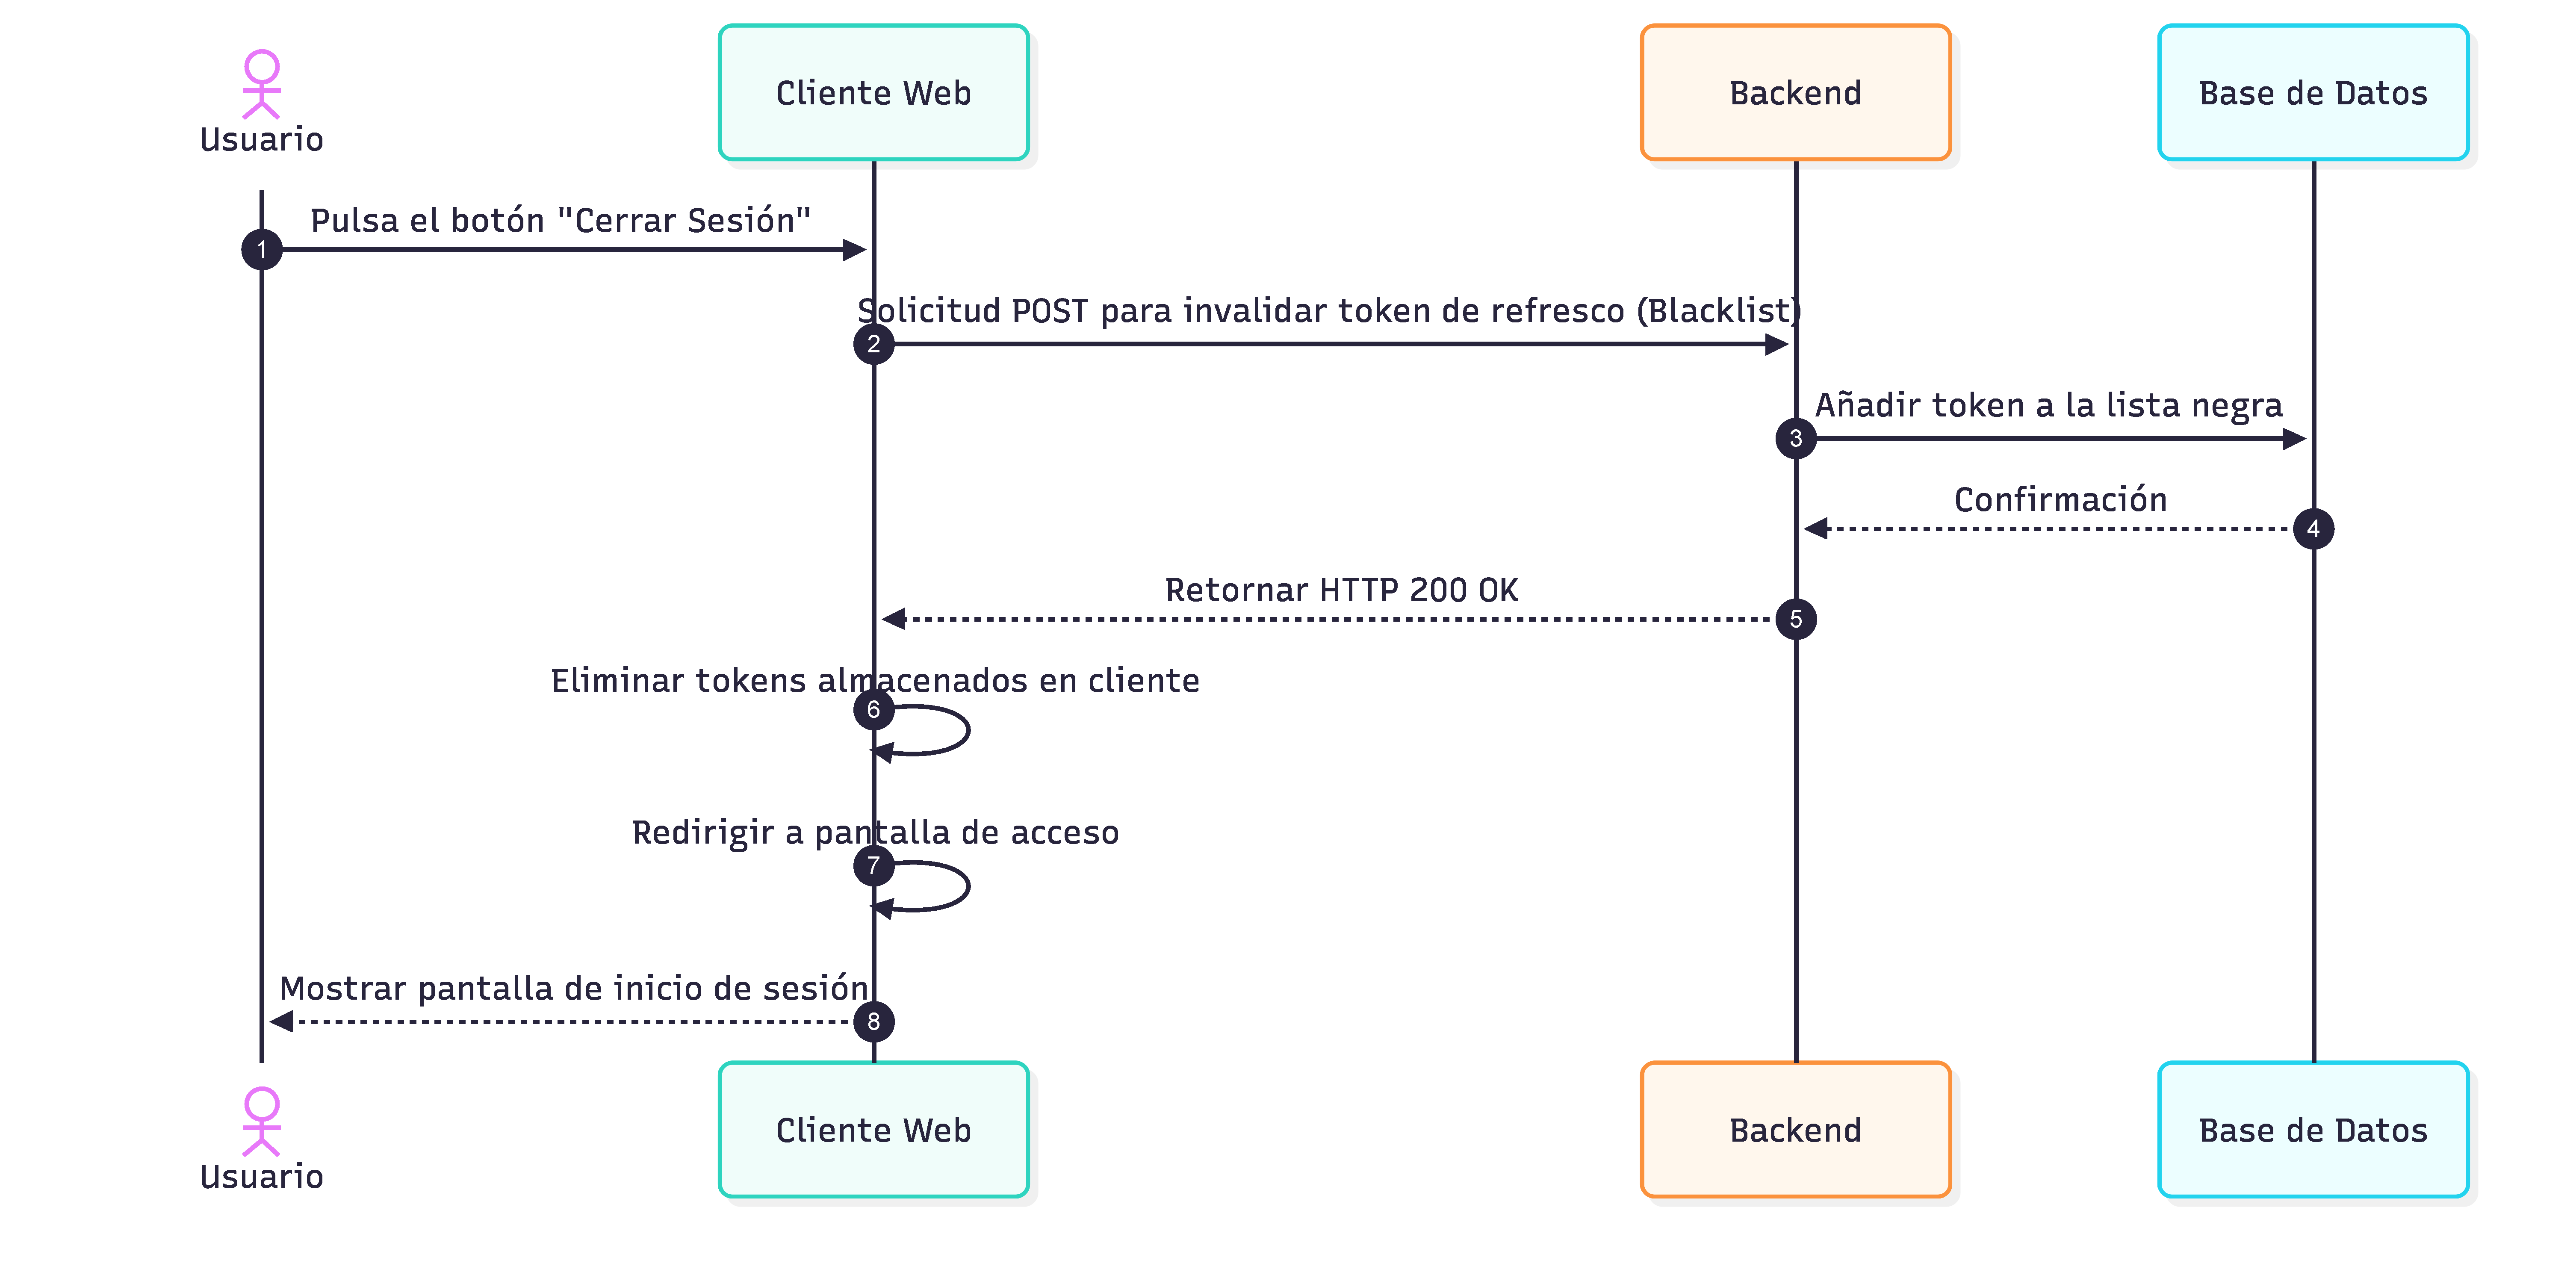
\includegraphics[width=0.85\textwidth]{./diagramas/secuencia_logout_SIMPLE.pdf}
\end{figure}

\begingroup
\shorthandoff{"<>"}
\setlength{\arrayrulewidth}{1pt}
\arrayrulecolor{vlepsbased}
\begin{longtable}{|p{15cm}|}
  \hline
  \rowcolor{maincolor} 
  \multicolumn{1}{|l|}{\textcolor{white}{\textbf{Caso de Uso}}} \\
  \hline
  \endfirsthead
  \multicolumn{1}{c}{{\tablename\ \thetable{} -- Continuación}} \\
  \hline
  \rowcolor{maincolor} 
  \multicolumn{1}{|l|}{\textcolor{white}{\textbf{Caso de Uso (Continuación)}}} \\
  \hline
  \endhead
  \hline \multicolumn{1}{|r|}{\textit{Continúa en la siguiente página...}} \\ \hline
  \endfoot
  \hline
  \caption{Caso de Uso CU7 — Modificación de datos del perfil.}
  \label{TB:CU7_PERFIL_DATOS}
  \endlastfoot

  \rowcolor{ulepsbased}
  \begin{tabularx}{\linewidth}{@{}X X@{}}
    \textbf{Identificador:} CU7 & \textbf{Actor principal:} Usuario
  \end{tabularx} \\ \hline

  \textbf{Nombre:} Modificación de datos del perfil \\ \hline

  \rowcolor{ulepsbased}
  \textbf{Descripción:} \newline 
  El usuario accede a la vista de ajustes para modificar su información personal (nombre de usuario y descripción/biografía). \\ \hline

  \textbf{Precondiciones:} \newline
  1. El usuario ha iniciado sesión. \\ \hline

  \rowcolor{ulepsbased}
  \textbf{Flujo principal:} \newline
  1. El usuario navega a la sección de "Perfil" desde la interfaz principal. \newline
  2. El sistema muestra los datos actuales del usuario (nombre de usuario, correo, descripción). \newline
  3. El usuario edita su nombre de usuario y/o descripción. \newline
  4. El usuario pulsa el botón "Guardar cambios". \newline
  5. El frontend envía una solicitud PATCH de actualización al backend con los datos modificados y su token de autenticación. \newline
  6. El sistema valida los permisos y verifica que el nuevo nombre de usuario no esté siendo utilizado por otra cuenta. \newline
  7. El sistema actualiza el registro en la base de datos de manera atómica. \newline
  8. El backend devuelve un código 200 OK con los datos actualizados. \newline
  9. La interfaz actualiza el estado local y muestra un aviso de éxito. \\ \hline

  \textbf{Flujos alternativos:} \newline
  \textbf{FA-01:} Nombre de usuario ya en uso: \newline
  1. Durante la actualización, el sistema detecta que el nombre de usuario solicitado ya pertenece a otro registro. \newline
  2. Se rechaza la modificación y el backend devuelve un error 400 Bad Request. \newline
  3. La interfaz muestra al usuario que el nombre no está disponible, abortando los cambios. \\ \hline

  \rowcolor{ulepsbased}
  \textbf{Postcondiciones:} \newline
  1. El nombre y la biografía del usuario se guardan actualizados en el sistema. \\ \hline

\end{longtable}
\endgroup

\begin{figure}[Diagrama de secuencia CU7]{FIG:CU7_SEQ}{Diagrama de secuencia de la modificación de datos del perfil.}
    \centering
    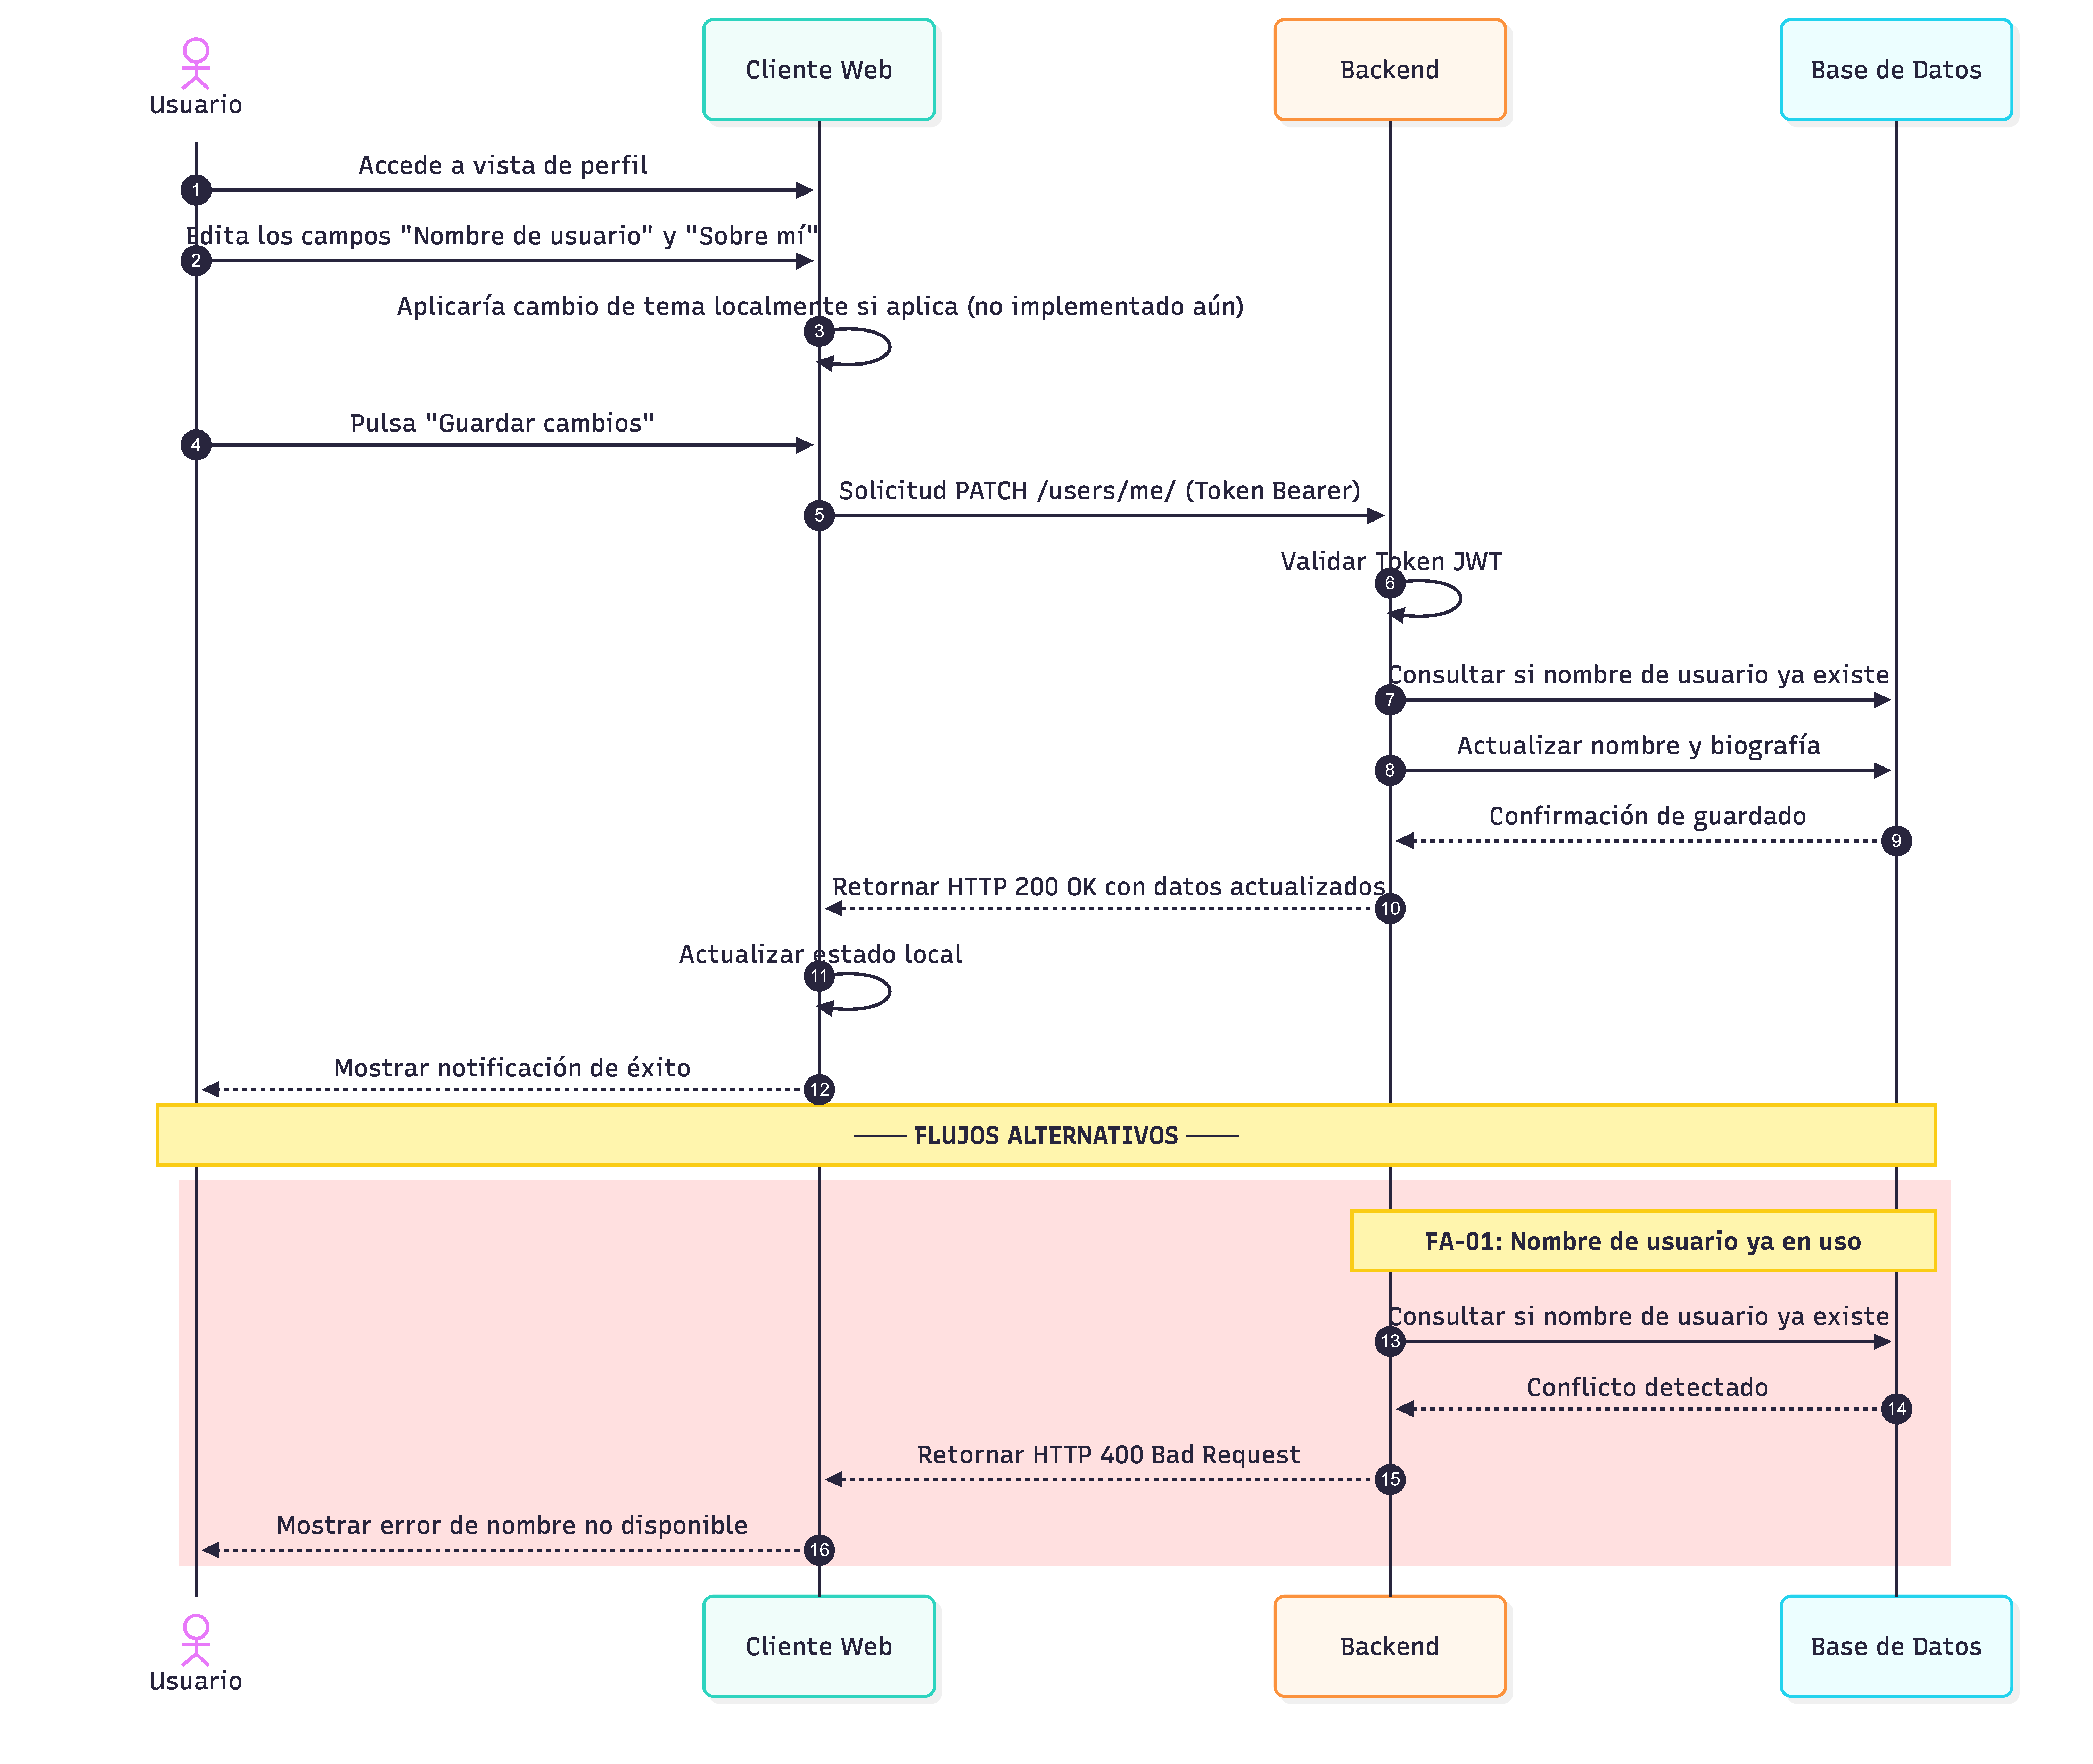
\includegraphics[width=0.85\textwidth]{./diagramas/secuencia_perfil_datos_SIMPLE.pdf}
\end{figure}

\begingroup
\shorthandoff{"<>"}
\setlength{\arrayrulewidth}{1pt}
\arrayrulecolor{vlepsbased}
\begin{longtable}{|p{15cm}|}
  \hline
  \rowcolor{maincolor} 
  \multicolumn{1}{|l|}{\textcolor{white}{\textbf{Caso de Uso}}} \\
  \hline
  \endfirsthead
  \multicolumn{1}{c}{{\tablename\ \thetable{} -- Continuación}} \\
  \hline
  \rowcolor{maincolor} 
  \multicolumn{1}{|l|}{\textcolor{white}{\textbf{Caso de Uso (Continuación)}}} \\
  \hline
  \endhead
  \hline \multicolumn{1}{|r|}{\textit{Continúa en la siguiente página...}} \\ \hline
  \endfoot
  \hline
  \caption{Caso de Uso CU8 — Cambio de contraseña.}
  \label{TB:CU8_PERFIL_PASSWORD}
  \endlastfoot

  \rowcolor{ulepsbased}
  \begin{tabularx}{\linewidth}{@{}X X@{}}
    \textbf{Identificador:} CU8 & \textbf{Actor principal:} Usuario
  \end{tabularx} \\ \hline

  \textbf{Nombre:} Cambio de contraseña \\ \hline

  \rowcolor{ulepsbased}
  \textbf{Descripción:} \newline 
  El usuario decide actualizar su contraseña de acceso desde su perfil introduciendo la clave actual y su nueva contraseña. \\ \hline

  \textbf{Precondiciones:} \newline
  1. El usuario ha iniciado sesión. \\ \hline

  \rowcolor{ulepsbased}
  \textbf{Flujo principal:} \newline
  1. El usuario navega a la sección de "Perfil" y selecciona la opción para cambiar contraseña. \newline
  2. El usuario introduce su contraseña actual y una nueva contraseña. \newline
  3. El usuario pulsa el botón de confirmación ("Cambiar contraseña"). \newline
  4. La interfaz envía una solicitud POST con las contraseñas al backend. \newline
  5. El sistema valida los permisos (mediante el token JWT) y comprueba las políticas de seguridad de la nueva clave. \newline
  6. El sistema verifica que la contraseña actual proporcionada coincida con el hash almacenado en la base de datos. \newline
  7. El sistema genera un nuevo hash para la contraseña y lo actualiza en la base de datos. \newline
  8. El backend retorna un código 204 confirmando la operación. \newline
  9. La interfaz muestra un aviso de éxito notificando el cambio de credenciales. \\ \hline

  \textbf{Flujos alternativos:} \newline
  \textbf{FA-01:} Contraseña actual incorrecta: \newline
  1. El sistema recupera el hash almacenado del usuario y comprueba que no coincide con la "contraseña actual" proporcionada. \newline
  2. Se rechaza la operación, retornando HTTP 400 Bad Request. \newline
  3. La interfaz informa al usuario de que sus credenciales son erróneas. \newline
  \textbf{FA-02:} Nueva contraseña inválida: \newline
  1. El backend detecta que la nueva contraseña no cumple con las políticas de seguridad mínimas (longitud, caracteres) o el frontend detecta que no coinciden (si hubiera confirmación). \newline
  2. Se aborta la operación con un error de validación (HTTP 400). \newline
  3. Se solicita al usuario que elija una contraseña diferente. \\ \hline

  \rowcolor{ulepsbased}
  \textbf{Postcondiciones:} \newline
  1. El hash de la contraseña del usuario se actualiza en el sistema y se requerirá la nueva clave en su próximo inicio de sesión. \\ \hline

\end{longtable}
\endgroup

\begin{figure}[Diagrama de secuencia CU8]{FIG:CU8_SEQ}{Diagrama de secuencia del cambio de contraseña.}
    \centering
    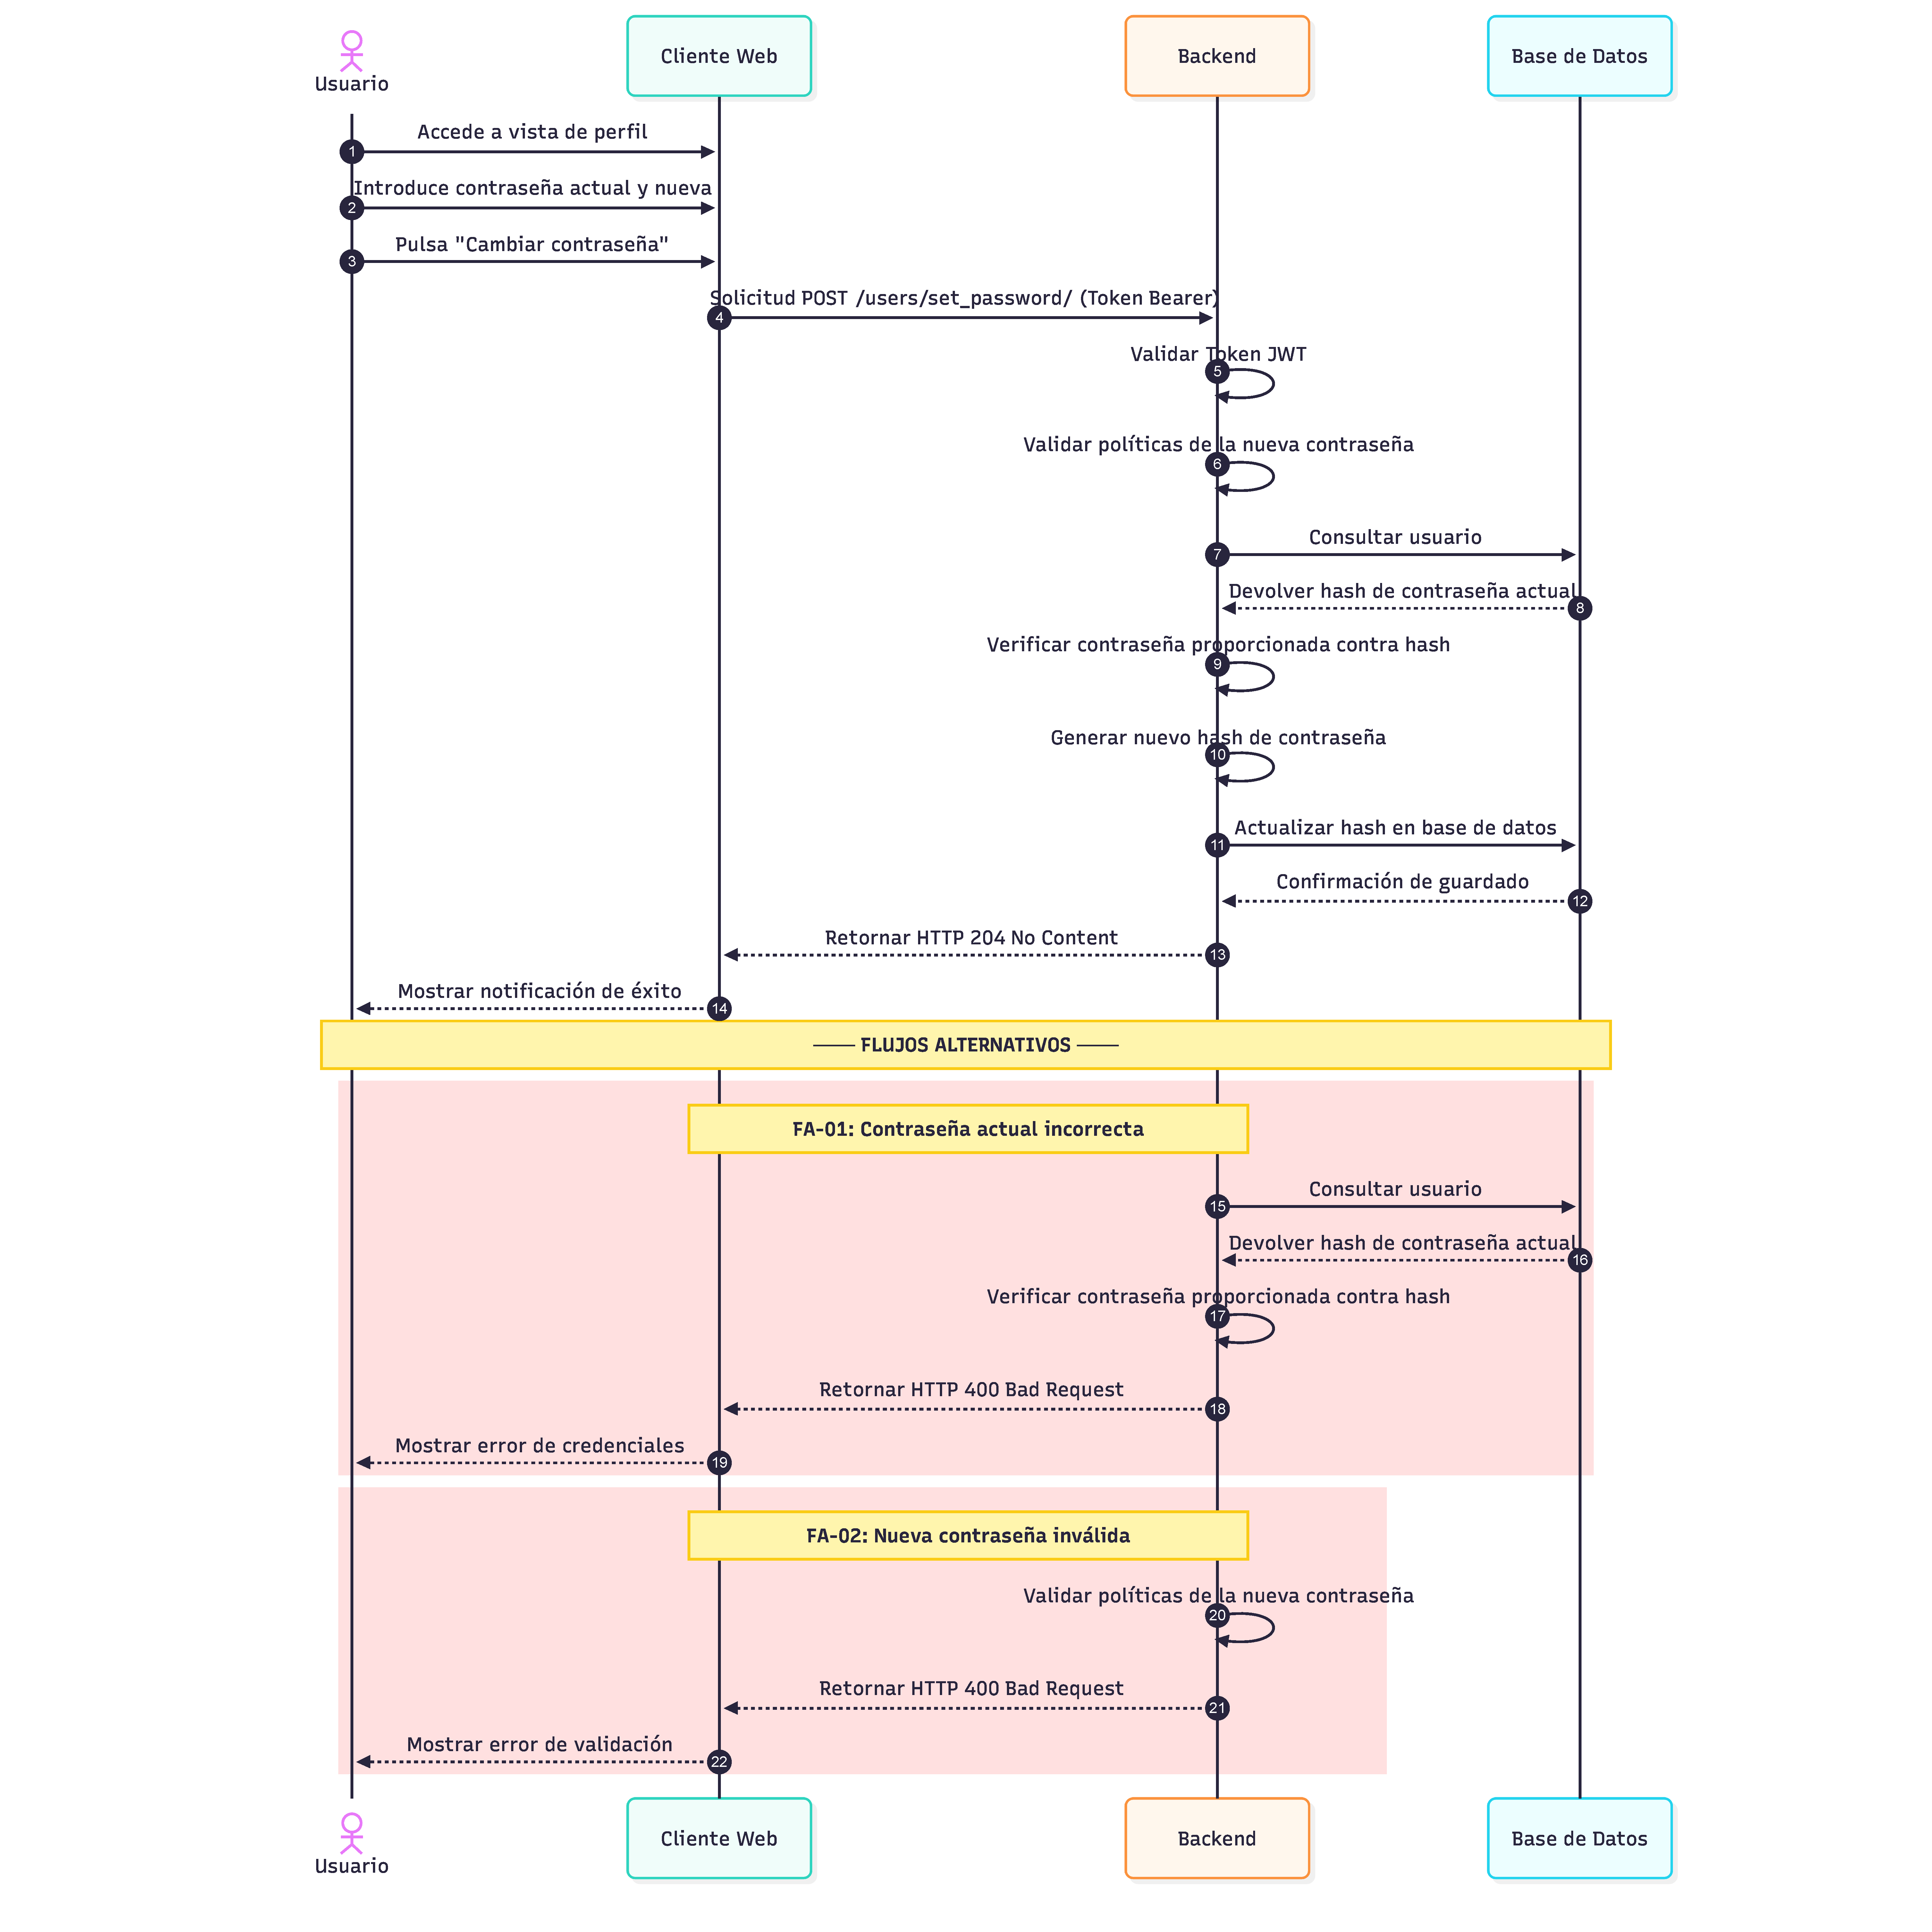
\includegraphics[width=0.85\textwidth]{./diagramas/secuencia_perfil_password_SIMPLE.pdf}
\end{figure}

\begingroup
\shorthandoff{"<>"}
\setlength{\arrayrulewidth}{1pt}
\arrayrulecolor{vlepsbased}
\begin{longtable}{|p{15cm}|}
  \hline
  \rowcolor{maincolor} 
  \multicolumn{1}{|l|}{\textcolor{white}{\textbf{Caso de Uso}}} \\
  \hline
  \endfirsthead
  \multicolumn{1}{c}{{\tablename\ \thetable{} -- Continuación}} \\
  \hline
  \rowcolor{maincolor} 
  \multicolumn{1}{|l|}{\textcolor{white}{\textbf{Caso de Uso (Continuación)}}} \\
  \hline
  \endhead
  \hline \multicolumn{1}{|r|}{\textit{Continúa en la siguiente página...}} \\ \hline
  \endfoot
  \hline
  \caption{Caso de Uso CU9 — Recuperación de contraseña olvidada.}
  \label{TB:CU9_RECUPERAR_PASSWORD}
  \endlastfoot

  \rowcolor{ulepsbased}
  \begin{tabularx}{\linewidth}{@{}X X@{}}
    \textbf{Identificador:} CU9 & \textbf{Actor principal:} Usuario no autenticado
  \end{tabularx} \\ \hline

  \textbf{Nombre:} Recuperación de contraseña olvidada \\ \hline

  \rowcolor{ulepsbased}
  \textbf{Descripción:} \newline 
  El usuario, al olvidar su contraseña, solicita un enlace temporal para poder crear una nueva clave y recuperar el acceso a su cuenta mediante el correo electrónico asociado. \\ \hline

  \textbf{Precondiciones:} \newline
  1. El sistema de envío de correos SMTP está configurado y operativo. \\ \hline

  \rowcolor{ulepsbased}
  \textbf{Flujo principal:} \newline
  1. El usuario accede a la opción "¿Olvidaste tu contraseña?" en la pantalla de acceso. \newline
  2. Introduce su dirección de correo electrónico y solicita la recuperación. \newline
  3. El sistema valida el formato e intenta localizar al usuario en la base de datos. \newline
  4. El sistema, por seguridad, devuelve una respuesta de confirmación idéntica independientemente de si el correo existe o no, para prevenir enumeración de cuentas. \newline
  5. En segundo plano, si el usuario existe, el sistema genera un token de un solo uso enlazado a dicho usuario y envía un correo electrónico. \newline
  6. El usuario accede a su bandeja de entrada, hace clic en el enlace, el cual le dirige a una vista especial en el frontend incluyendo los parámetros (UID y Token). \newline
  7. El usuario introduce una nueva contraseña segura y confirma. \newline
  8. El frontend envía la nueva clave al backend junto al UID y Token. \newline
  9. El sistema valida el token (que no haya expirado ni sido usado). \newline
  10. El sistema actualiza el hash de la contraseña en la base de datos. \newline
  11. Se informa al usuario y se le redirige al inicio de sesión. \\ \hline

  \textbf{Flujos alternativos:} \newline
  \textbf{FA-01:} Token inválido o expirado: \newline
  1. En el paso 9, el sistema detecta que el token ha expirado o que ya fue utilizado previamente. \newline
  2. Se rechaza la petición con un error HTTP 400. \newline
  3. El frontend muestra un mensaje indicando que el enlace ya no es válido y requiere solicitar uno nuevo. \\ \hline

  \rowcolor{ulepsbased}
  \textbf{Postcondiciones:} \newline
  1. La contraseña anterior es revocada y la nueva entra en funcionamiento. \newline
  2. El token de recuperación queda inmediatamente invalidado. \\ \hline

\end{longtable}
\endgroup

\begin{figure}[Diagrama de secuencia CU9]{FIG:CU9_SEQ}{Diagrama de secuencia de la recuperación de contraseña.}
    \centering
    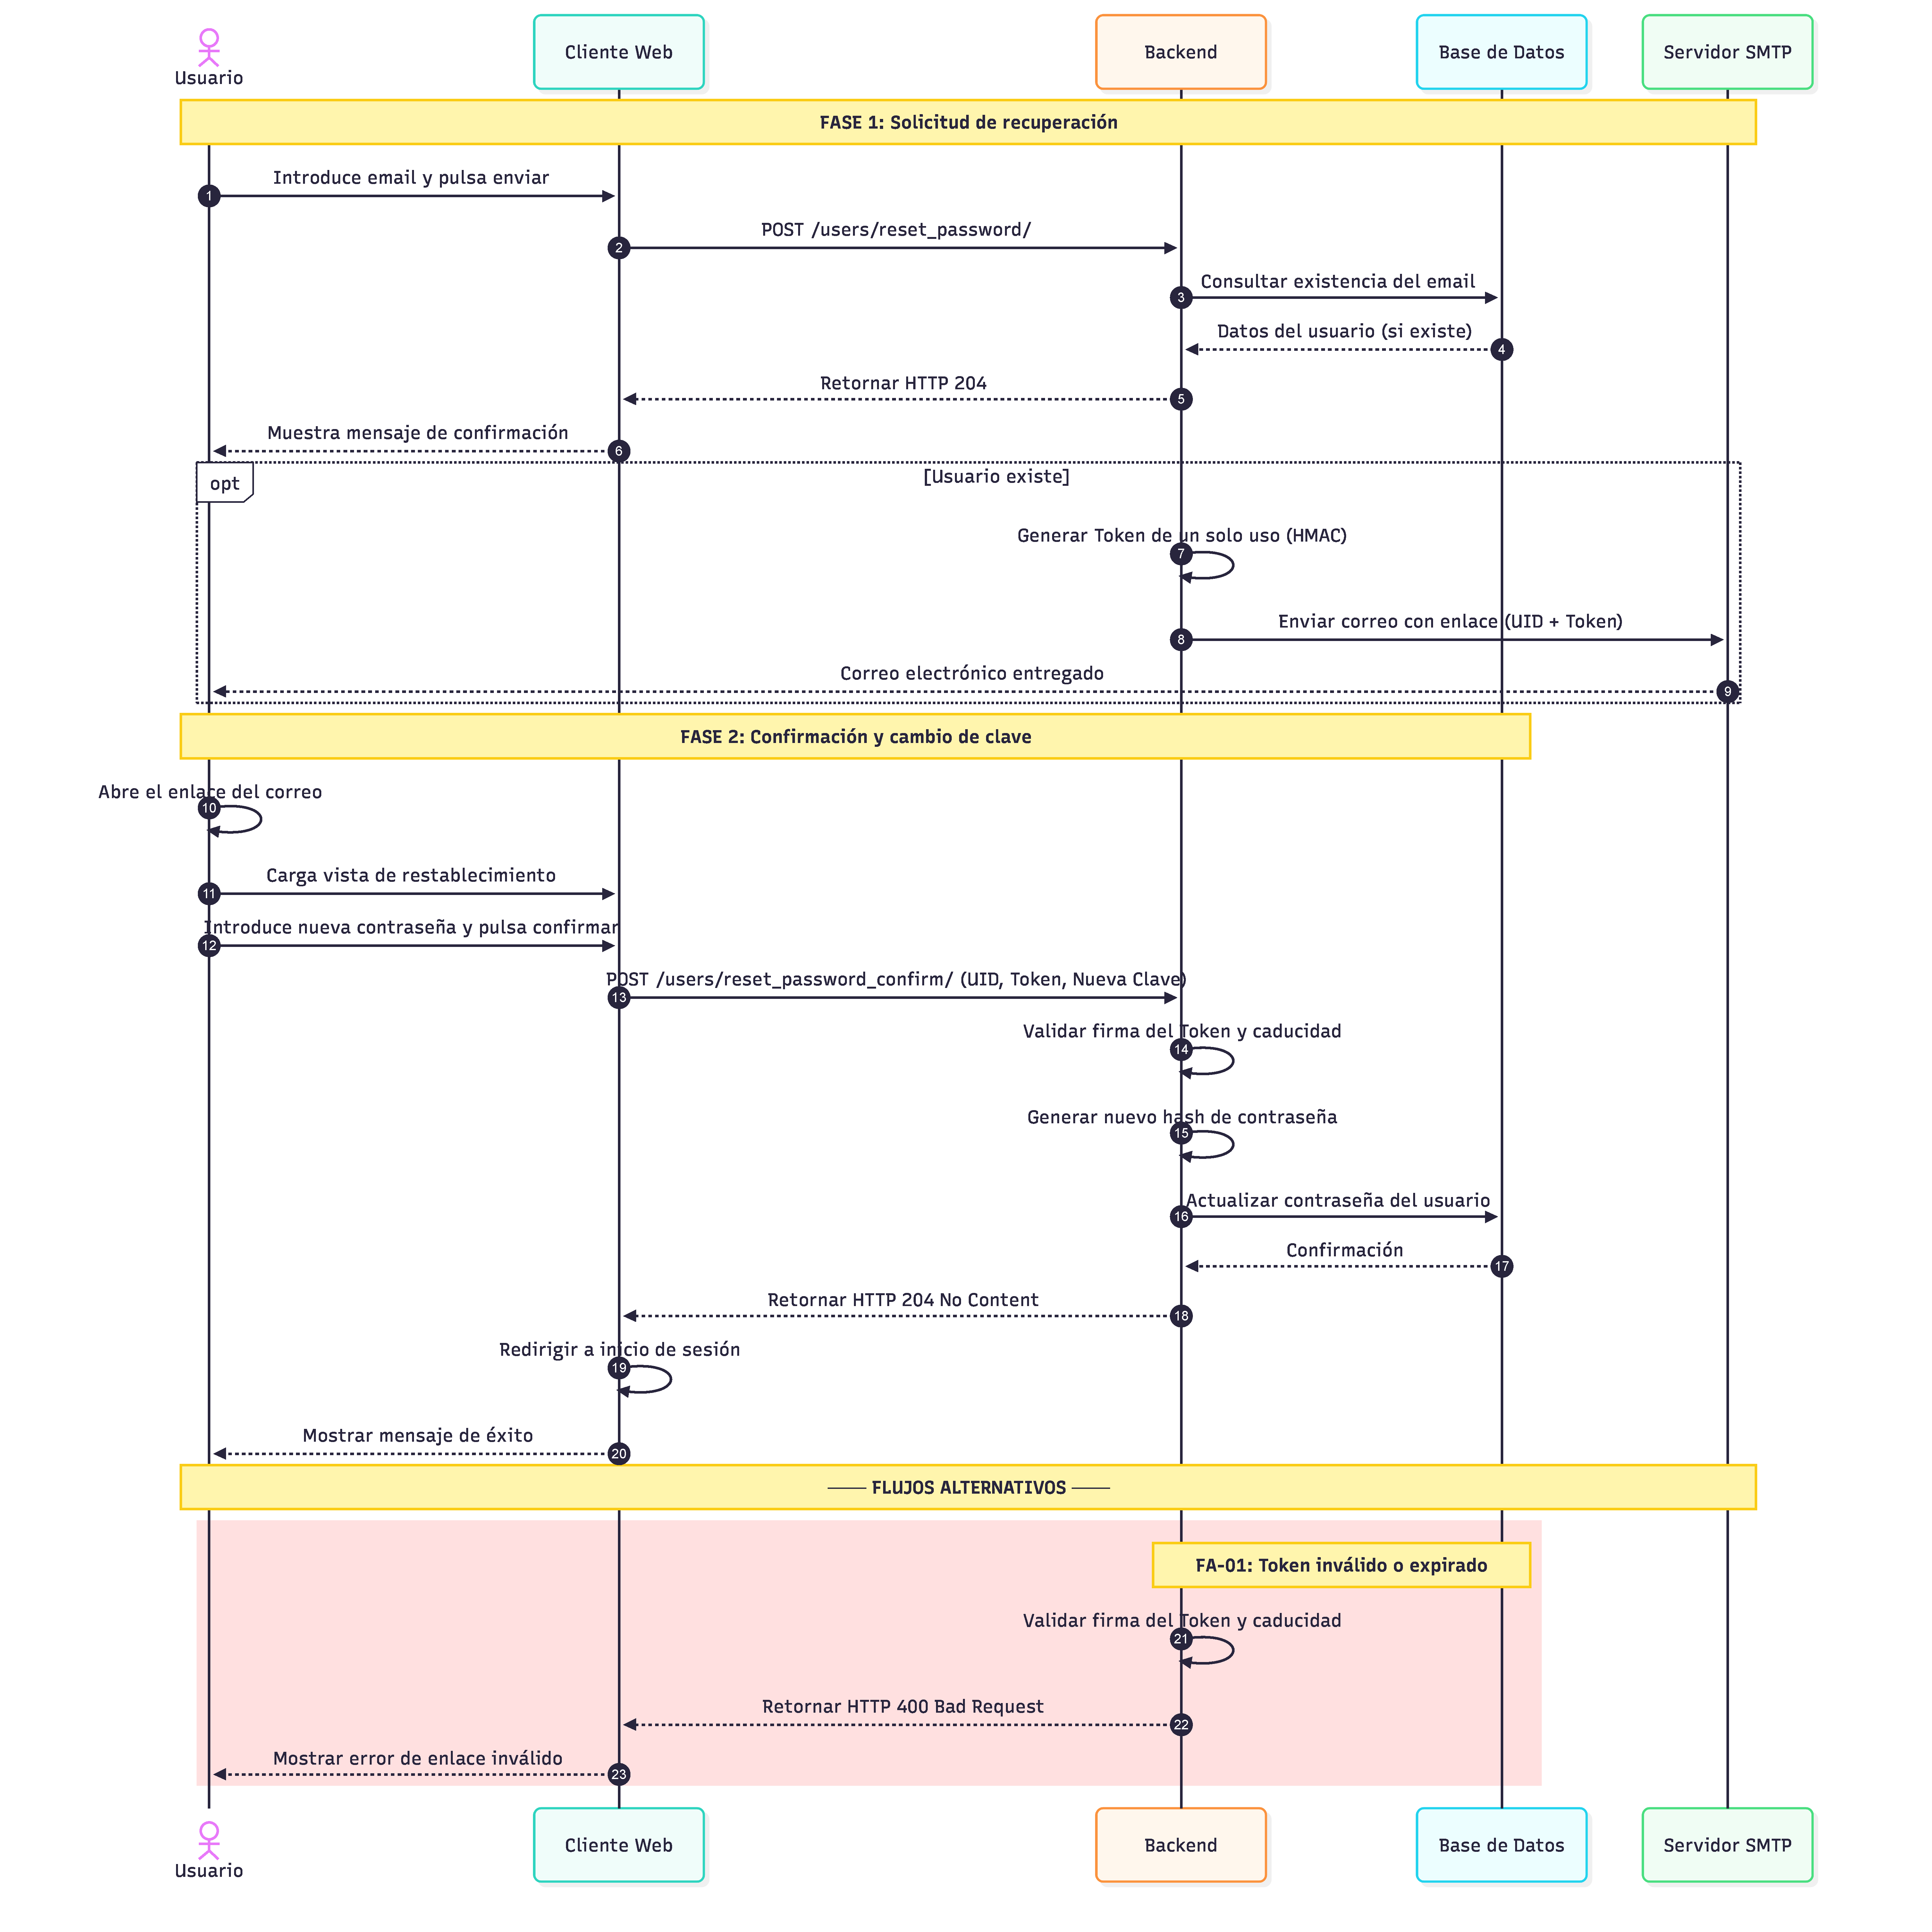
\includegraphics[width=0.85\textwidth]{./diagramas/secuencia_recuperar_password_SIMPLE.pdf}
\end{figure}

\begingroup
\shorthandoff{"<>"}
\setlength{\arrayrulewidth}{1pt}
\arrayrulecolor{vlepsbased}
\begin{longtable}{|p{15cm}|}
  \hline
  \rowcolor{maincolor} 
  \multicolumn{1}{|l|}{\textcolor{white}{\textbf{Caso de Uso}}} \\
  \hline
  \endfirsthead
  \multicolumn{1}{c}{{\tablename\ \thetable{} -- Continuación}} \\
  \hline
  \rowcolor{maincolor} 
  \multicolumn{1}{|l|}{\textcolor{white}{\textbf{Caso de Uso (Continuación)}}} \\
  \hline
  \endhead
  \hline \multicolumn{1}{|r|}{\textit{Continúa en la siguiente página...}} \\ \hline
  \endfoot
  \hline
  \caption{Caso de Uso CU10 — Renombrado manual de sesión de chat.}
  \label{TB:CU10_RENOMBRAR_SESION}
  \endlastfoot

  \rowcolor{ulepsbased}
  \begin{tabularx}{\linewidth}{@{}X X@{}}
    \textbf{Identificador:} CU10 & \textbf{Actor principal:} Usuario
  \end{tabularx} \\ \hline

  \textbf{Nombre:} Renombrado manual de sesión de chat \\ \hline

  \rowcolor{ulepsbased}
  \textbf{Descripción:} \newline 
  El usuario decide modificar el título de una sesión de chat existente en su panel lateral para facilitar su organización, introduciendo un nuevo nombre. \\ \hline

  \textbf{Precondiciones:} \newline
  1. El usuario ha iniciado sesión. \newline
  2. Existe al menos una sesión de chat en su historial. \\ \hline

  \rowcolor{ulepsbased}
  \textbf{Flujo principal:} \newline
  1. El usuario hace clic en el botón de "Renombrar" junto a la sesión deseada en el panel lateral. \newline
  2. La interfaz reemplaza el título estático por un campo de texto editable y solicita el nuevo título. \newline
  3. El usuario escribe el nuevo nombre y confirma (pulsando Enter o el botón de guardado). \newline
  4. La interfaz valida que el campo de texto no esté vacío ni compuesto solo por espacios en blanco. \newline
  5. La interfaz envía la petición al backend con el nuevo título. \newline
  6. El backend verifica la propiedad de la sesión y comprueba que el título no llegue vacío. \newline
  7. Si el título supera los 200 caracteres, el backend realiza un truncado silencioso recortándolo al límite permitido. \newline
  8. El sistema actualiza el título en la base de datos y devuelve el título modificado exitosamente. \newline
  9. El frontend actualiza el nombre visualmente en el panel lateral. \\ \hline

  \textbf{Flujos alternativos:} \newline
  \textbf{FA-01:} Título vacío o en blanco: \newline
  1. El sistema detecta en el frontend que el título introducido está vacío o contiene únicamente espacios en blanco. \newline
  2. La función de guardado se aborta sin llegar a enviar ninguna solicitud HTTP al backend. \newline
  3. La interfaz cancela el modo de edición silenciosamente y restaura el título original. \\ \hline

  \rowcolor{ulepsbased}
  \textbf{Postcondiciones:} \newline
  1. El nuevo título queda asociado a la sesión en la base de datos de manera permanente. \\ \hline

\end{longtable}
\endgroup

\begin{figure}[Diagrama de secuencia CU10]{FIG:CU10_SEQ}{Diagrama de secuencia del renombrado de sesión.}
    \centering
    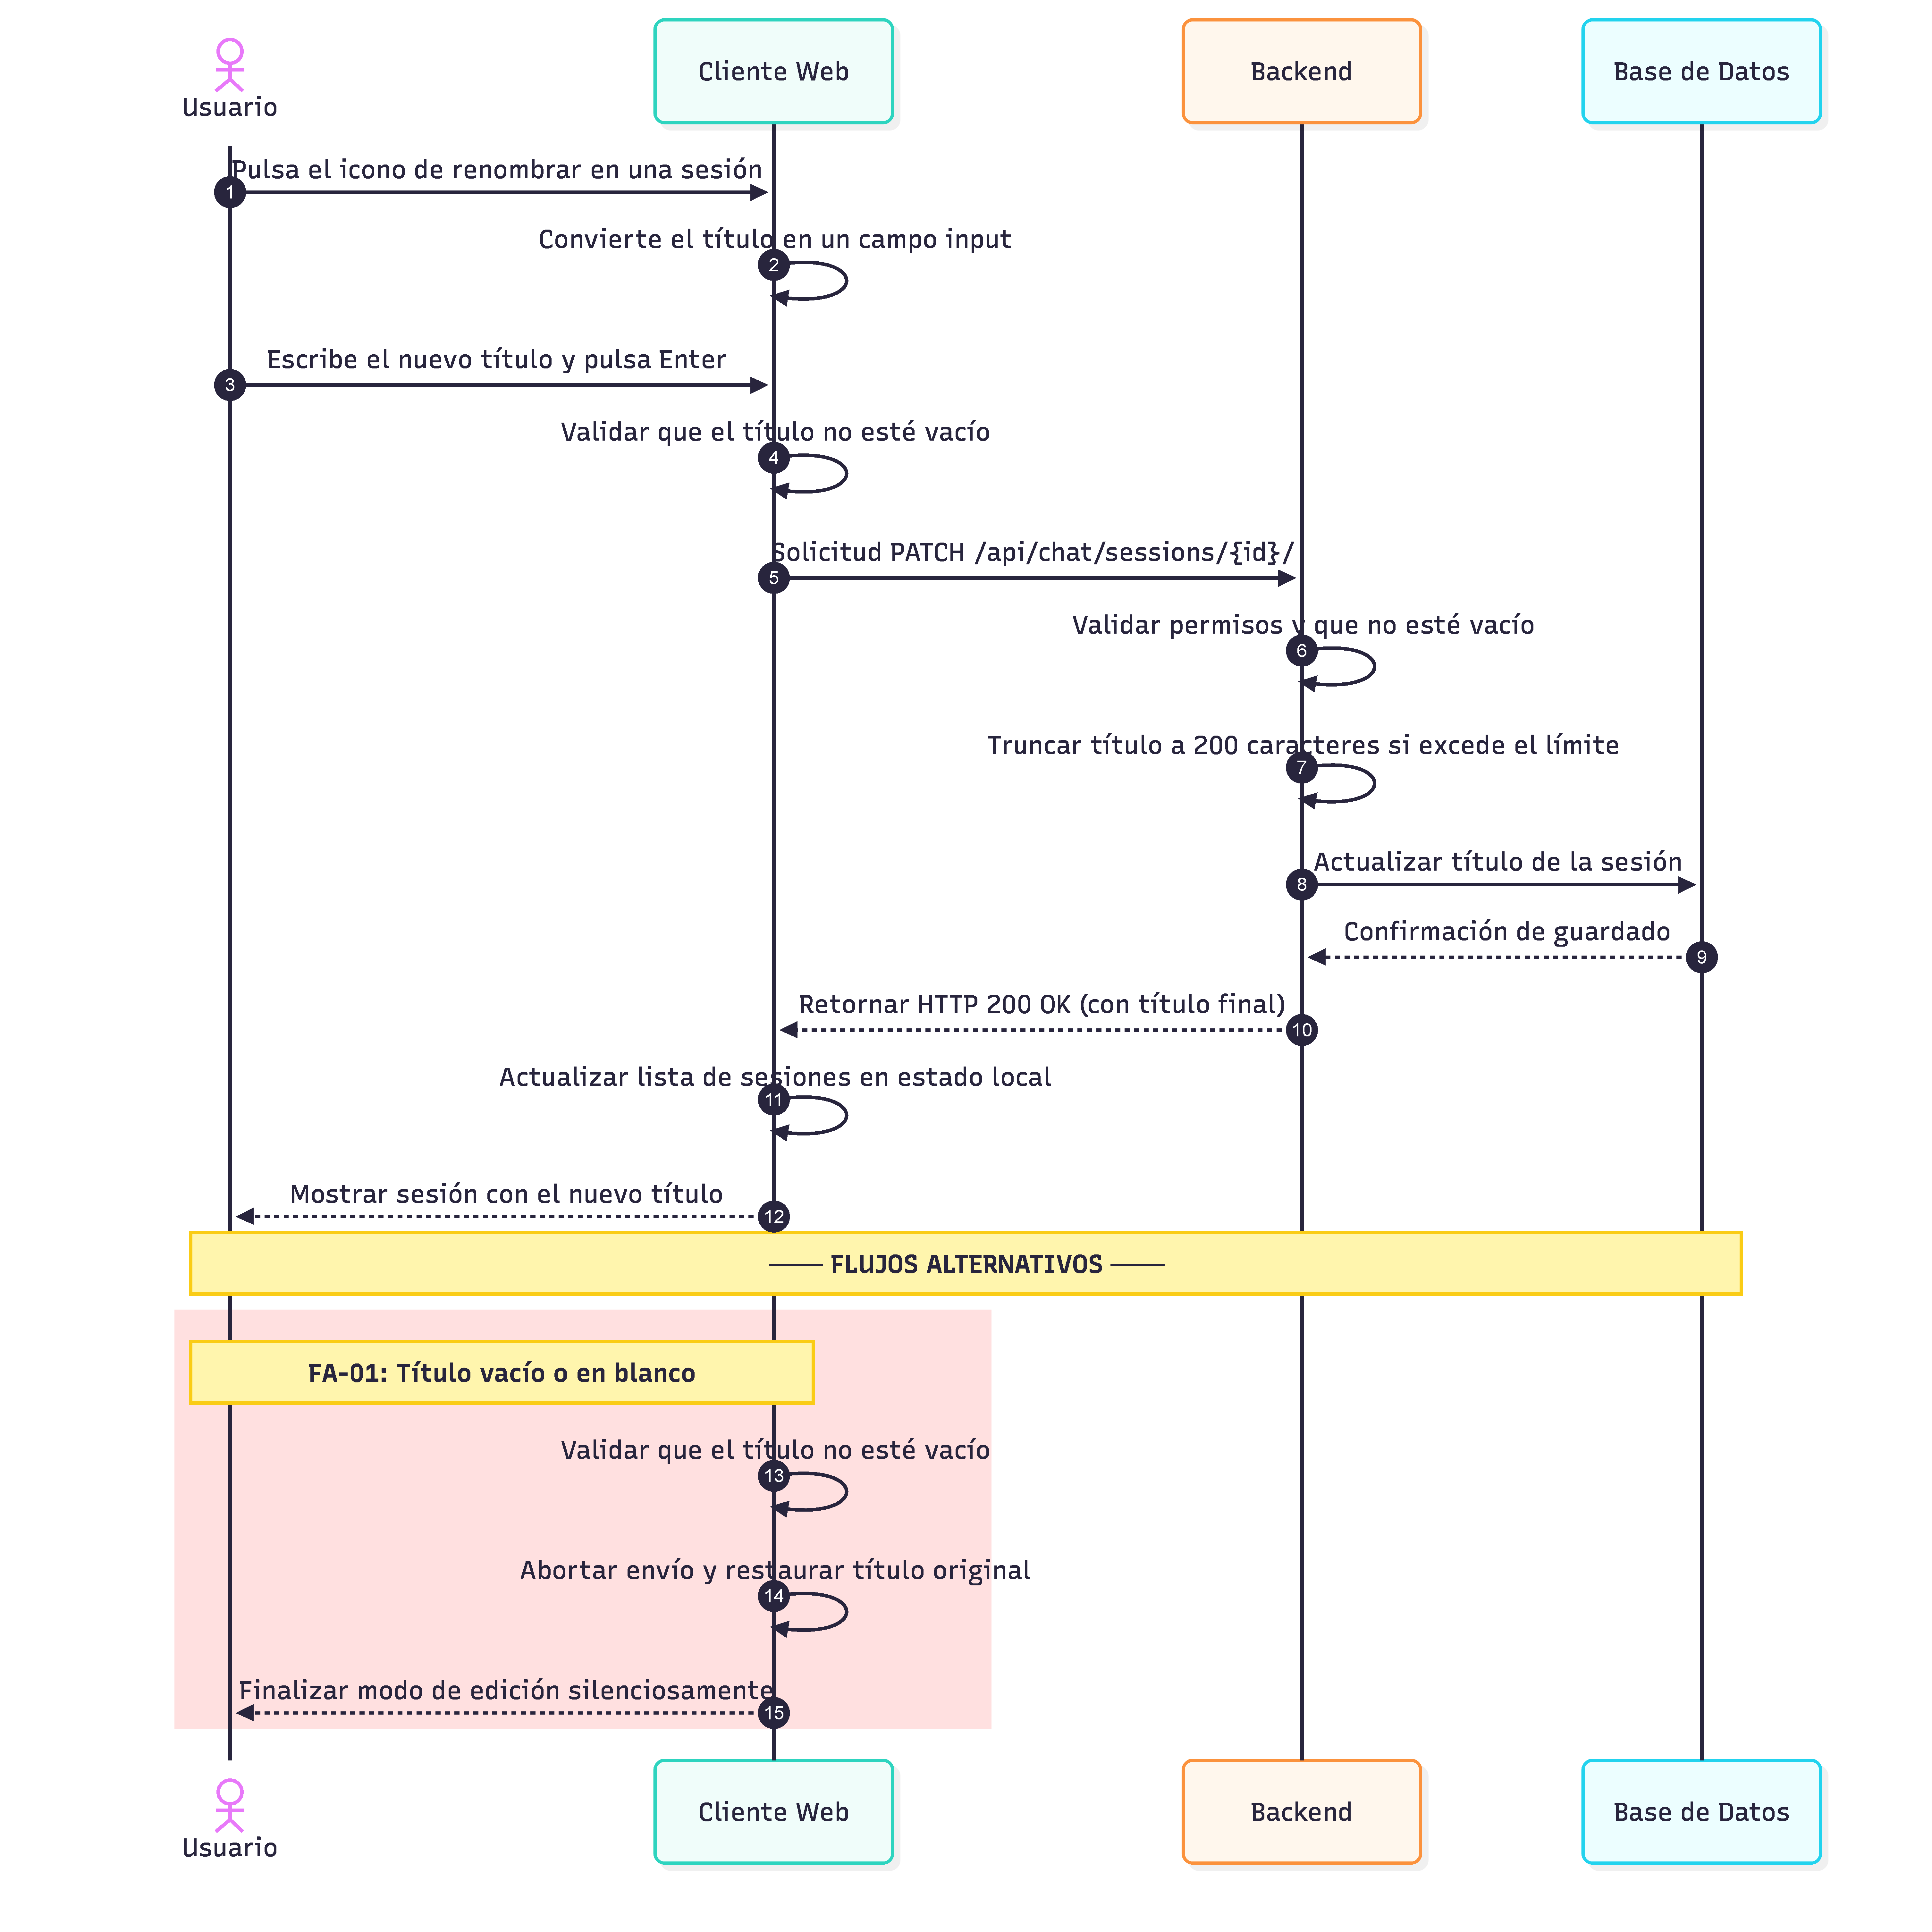
\includegraphics[width=0.85\textwidth]{./diagramas/secuencia_renombrar_sesion_SIMPLE.pdf}
\end{figure}

\begingroup
\shorthandoff{"<>"}
\setlength{\arrayrulewidth}{1pt}
\arrayrulecolor{vlepsbased}
\begin{longtable}{|p{15cm}|}
  \hline
  \rowcolor{maincolor} 
  \multicolumn{1}{|l|}{\textcolor{white}{\textbf{Caso de Uso}}} \\
  \hline
  \endfirsthead
  \multicolumn{1}{c}{{\tablename\ \thetable{} -- Continuación}} \\
  \hline
  \rowcolor{maincolor} 
  \multicolumn{1}{|l|}{\textcolor{white}{\textbf{Caso de Uso (Continuación)}}} \\
  \hline
  \endhead
  \hline \multicolumn{1}{|r|}{\textit{Continúa en la siguiente página...}} \\ \hline
  \endfoot
  \hline
  \caption{Caso de Uso CU11 — Eliminación permanente de sesión de chat.}
  \label{TB:CU11_ELIMINAR_SESION}
  \endlastfoot

  \rowcolor{ulepsbased}
  \begin{tabularx}{\linewidth}{@{}X X@{}}
    \textbf{Identificador:} CU11 & \textbf{Actor principal:} Usuario
  \end{tabularx} \\ \hline

  \textbf{Nombre:} Eliminación permanente de sesión de chat \\ \hline

  \rowcolor{ulepsbased}
  \textbf{Descripción:} \newline 
  El usuario decide eliminar permanentemente una sesión de chat completa de su historial, provocando el borrado de todos los mensajes asociados a la misma. \\ \hline

  \textbf{Precondiciones:} \newline
  1. El usuario ha iniciado sesión. \newline
  2. Existe al menos una sesión de chat. \\ \hline

  \rowcolor{ulepsbased}
  \textbf{Flujo principal:} \newline
  1. El usuario hace clic en el botón de eliminar (ícono de papelera) junto a una sesión en el panel lateral. \newline
  2. El frontend muestra un cuadro de diálogo de confirmación (¿Eliminar esta conversación? Esta acción no se puede deshacer.). \newline
  3. El usuario confirma la eliminación. \newline
  4. La interfaz envía una solicitud HTTP DELETE al backend. \newline
  5. El sistema verifica la propiedad y borra el registro de la sesión y, en cascada, todos sus mensajes asociados en la base de datos. \newline
  6. El sistema devuelve HTTP 204 (No Content). \newline
  7. El frontend elimina la sesión de la lista visual y, si el usuario estaba visualizando la sesión eliminada, limpia la pantalla y lo devuelve a la vista inicial (pantalla de creación de "Nueva conversación"), independientemente de si hay más sesiones en el historial. \\ \hline

  \textbf{Flujos alternativos:} \newline
  \textbf{FA-01:} Cancelación del borrado: \newline
  1. En el paso 2, el usuario pulsa "Cancelar". \newline
  2. Se cierra el cuadro de diálogo y no se envía ninguna solicitud al backend. \\ \hline

  \rowcolor{ulepsbased}
  \textbf{Postcondiciones:} \newline
  1. La sesión y todo su historial de mensajes desaparecen permanentemente del sistema. \\ \hline

\end{longtable}
\endgroup

\begin{figure}[Diagrama de secuencia CU11]{FIG:CU11_SEQ}{Diagrama de secuencia de la eliminación de sesión.}
    \centering
    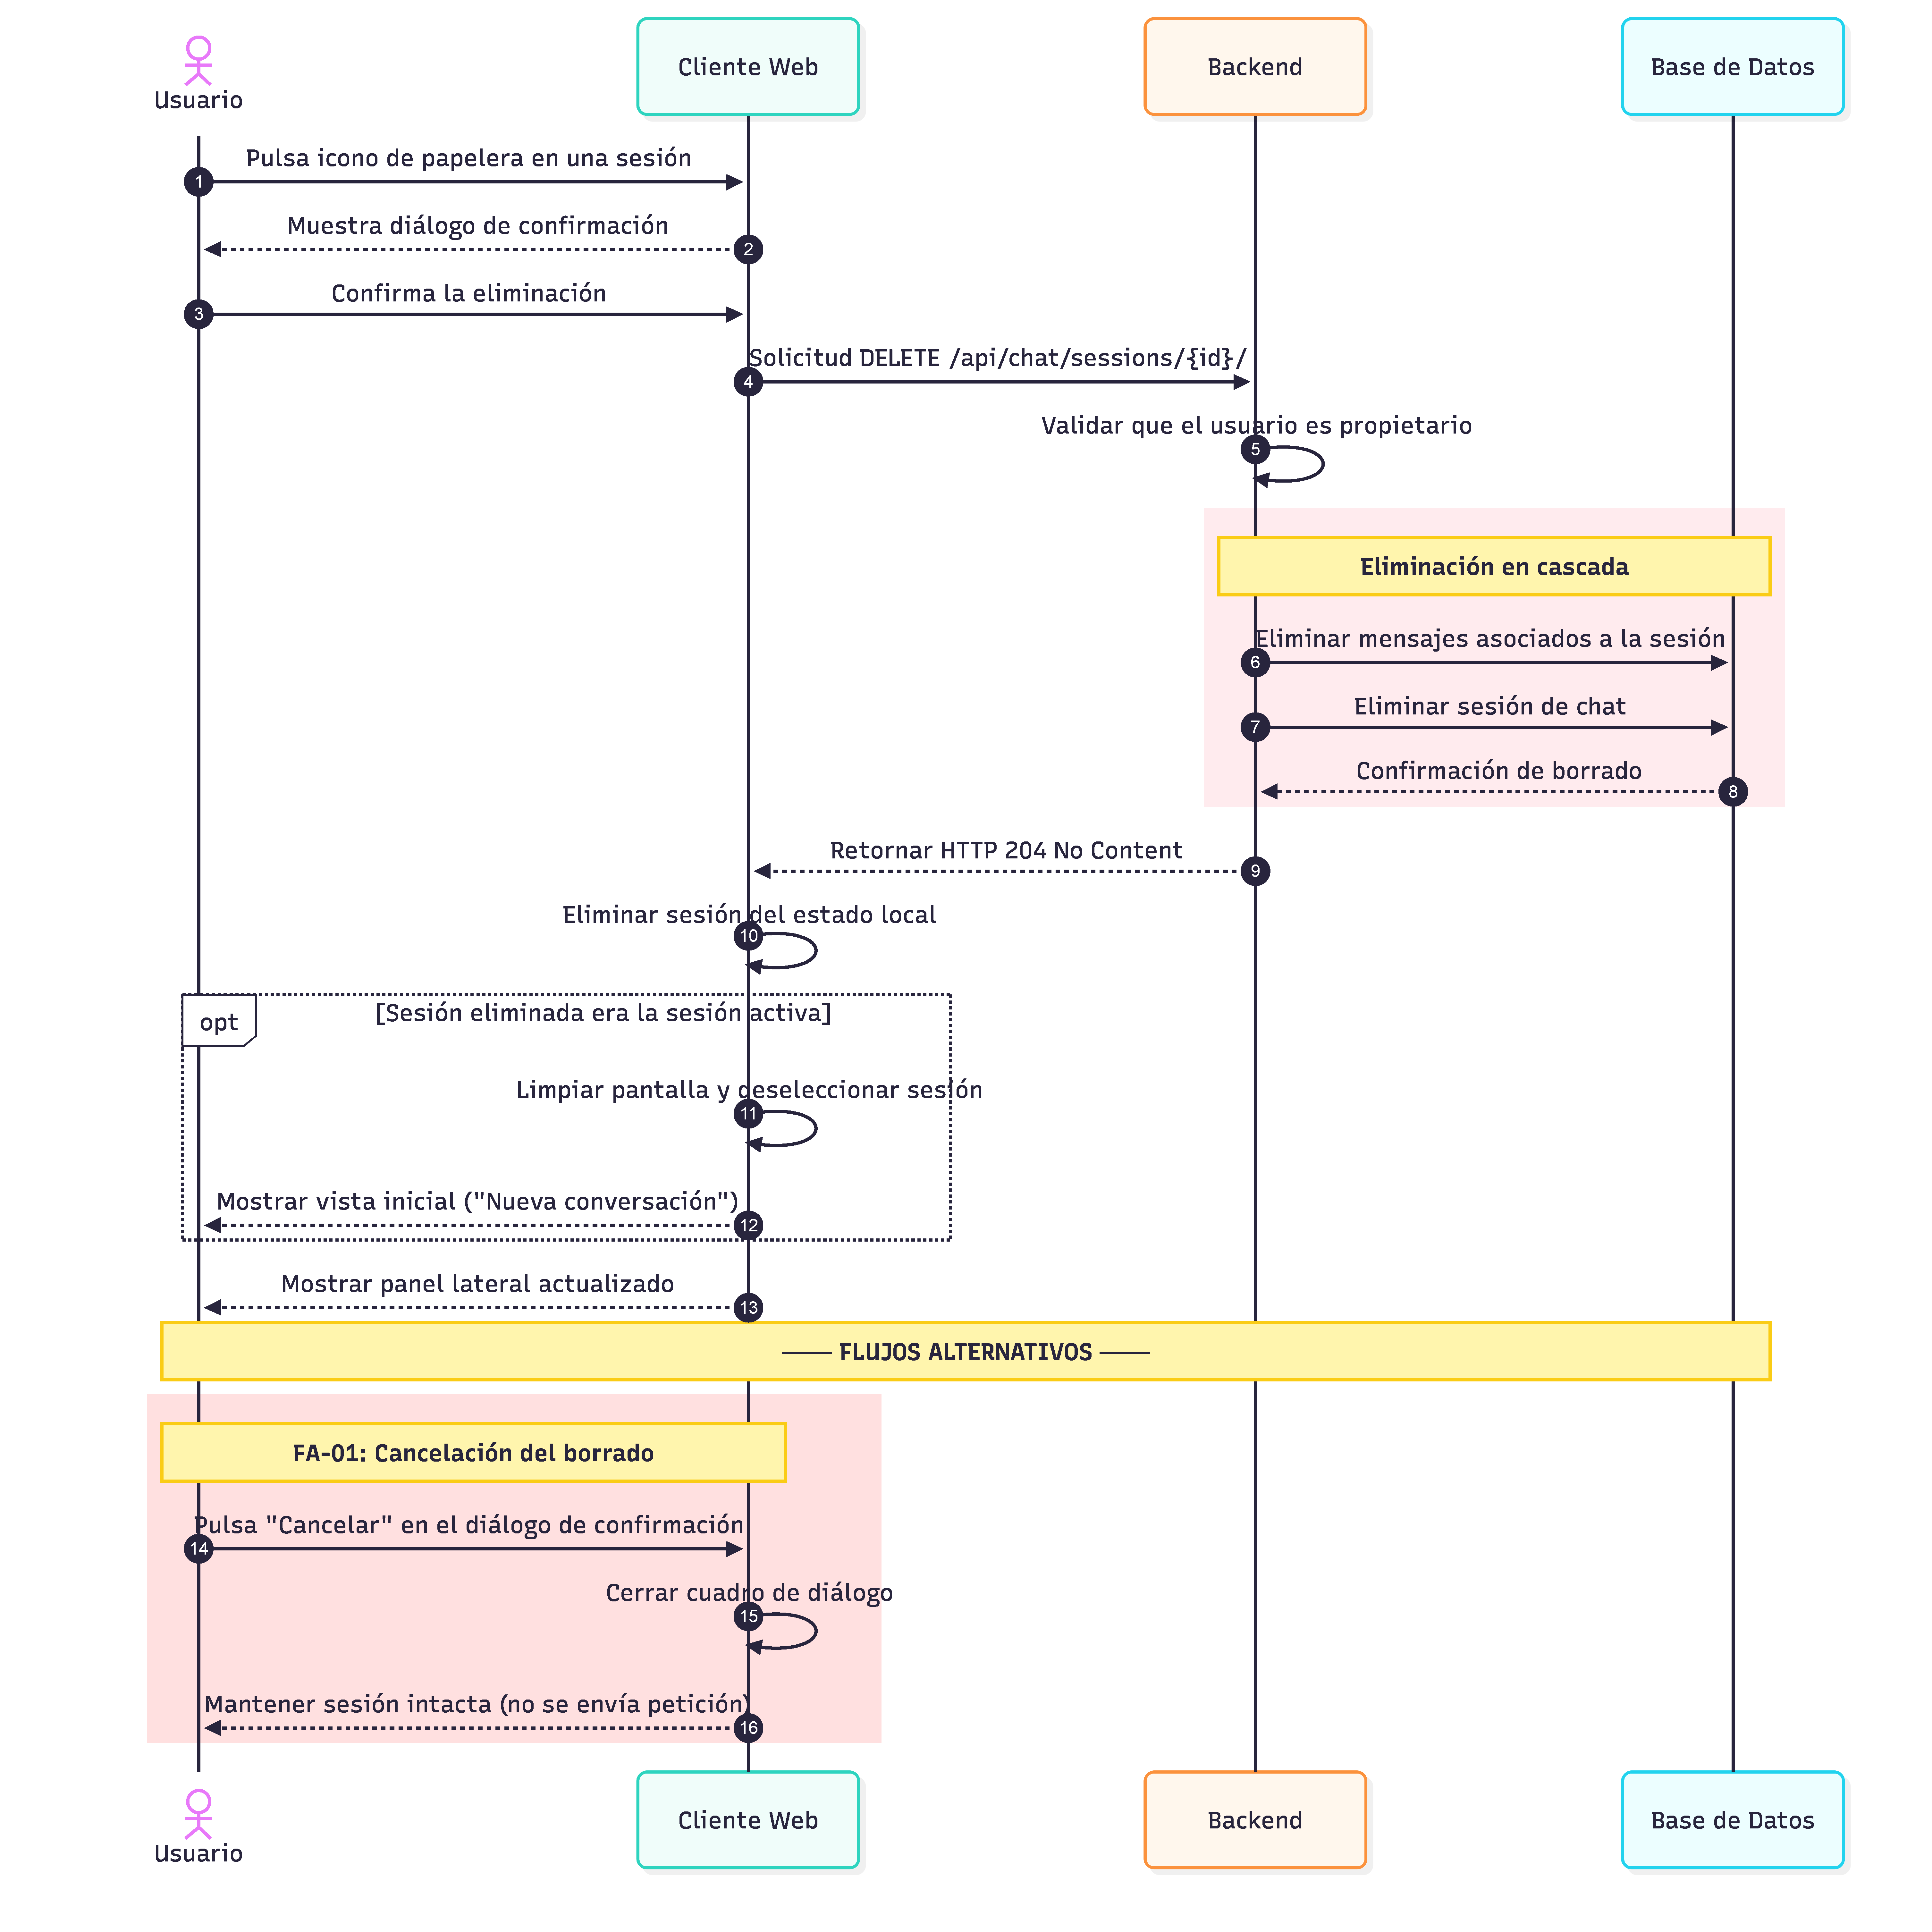
\includegraphics[width=0.85\textwidth]{./diagramas/secuencia_eliminar_sesion_SIMPLE.pdf}
\end{figure}

\begingroup
\shorthandoff{"<>"}
\setlength{\arrayrulewidth}{1pt}
\arrayrulecolor{vlepsbased}
\begin{longtable}{|p{15cm}|}
  \hline
  \rowcolor{maincolor} 
  \multicolumn{1}{|l|}{\textcolor{white}{\textbf{Caso de Uso}}} \\
  \hline
  \endfirsthead
  \multicolumn{1}{c}{{\tablename\ \thetable{} -- Continuación}} \\
  \hline
  \rowcolor{maincolor} 
  \multicolumn{1}{|l|}{\textcolor{white}{\textbf{Caso de Uso (Continuación)}}} \\
  \hline
  \endhead
  \hline \multicolumn{1}{|r|}{\textit{Continúa en la siguiente página...}} \\ \hline
  \endfoot
  \hline
  \caption{Caso de Uso CU12 — Consulta del historial de sesiones y mensajes.}
  \label{TB:CU12_HISTORIAL}
  \endlastfoot

  \rowcolor{ulepsbased}
  \begin{tabularx}{\linewidth}{@{}X X@{}}
    \textbf{Identificador:} CU12 & \textbf{Actor principal:} Usuario
  \end{tabularx} \\ \hline

  \textbf{Nombre:} Consulta del historial de sesiones y mensajes \\ \hline

  \rowcolor{ulepsbased}
  \textbf{Descripción:} \newline 
  El usuario accede a la plataforma y recupera automáticamente la lista de sus sesiones pasadas. Al seleccionar una, el sistema recupera todos los mensajes asociados y los visualiza cronológicamente en el chat. \\ \hline

  \textbf{Precondiciones:} \newline
  1. El usuario ha iniciado sesión y existen sesiones en su cuenta. \\ \hline

  \rowcolor{ulepsbased}
  \textbf{Flujo principal:} \newline
  1. El usuario accede a la interfaz principal de la aplicación. \newline
  2. El frontend solicita el listado paginado de sesiones asociadas a la cuenta. \newline
  3. El backend valida la autenticación y retorna los registros ordenados por fecha de última actualización. \newline
  4. La interfaz pinta este historial de conversaciones en el panel lateral. \newline
  5. El usuario hace clic sobre una de las sesiones anteriores. \newline
  6. El frontend envía una petición al backend para obtener los mensajes de esa sesión concreta. \newline
  7. El backend devuelve la lista de mensajes ordenados cronológicamente (con su contenido, remitente y fecha). \newline
  8. La interfaz principal limpia la vista actual y renderiza el historial recuperado, permitiendo al usuario retomar la conversación o revisarla. \\ \hline

  \rowcolor{ulepsbased}
  \textbf{Postcondiciones:} \newline
  1. El estado activo de la interfaz se sincroniza con la sesión seleccionada, preparándose para recibir nuevos mensajes (enlaza con el CU1). \\ \hline

  \textbf{Flujos alternativos:} \newline
  Ninguno. \\ \hline

\end{longtable}
\endgroup

\begin{figure}[Diagrama de secuencia CU12]{FIG:CU12_SEQ}{Diagrama de secuencia del historial.}
    \centering
    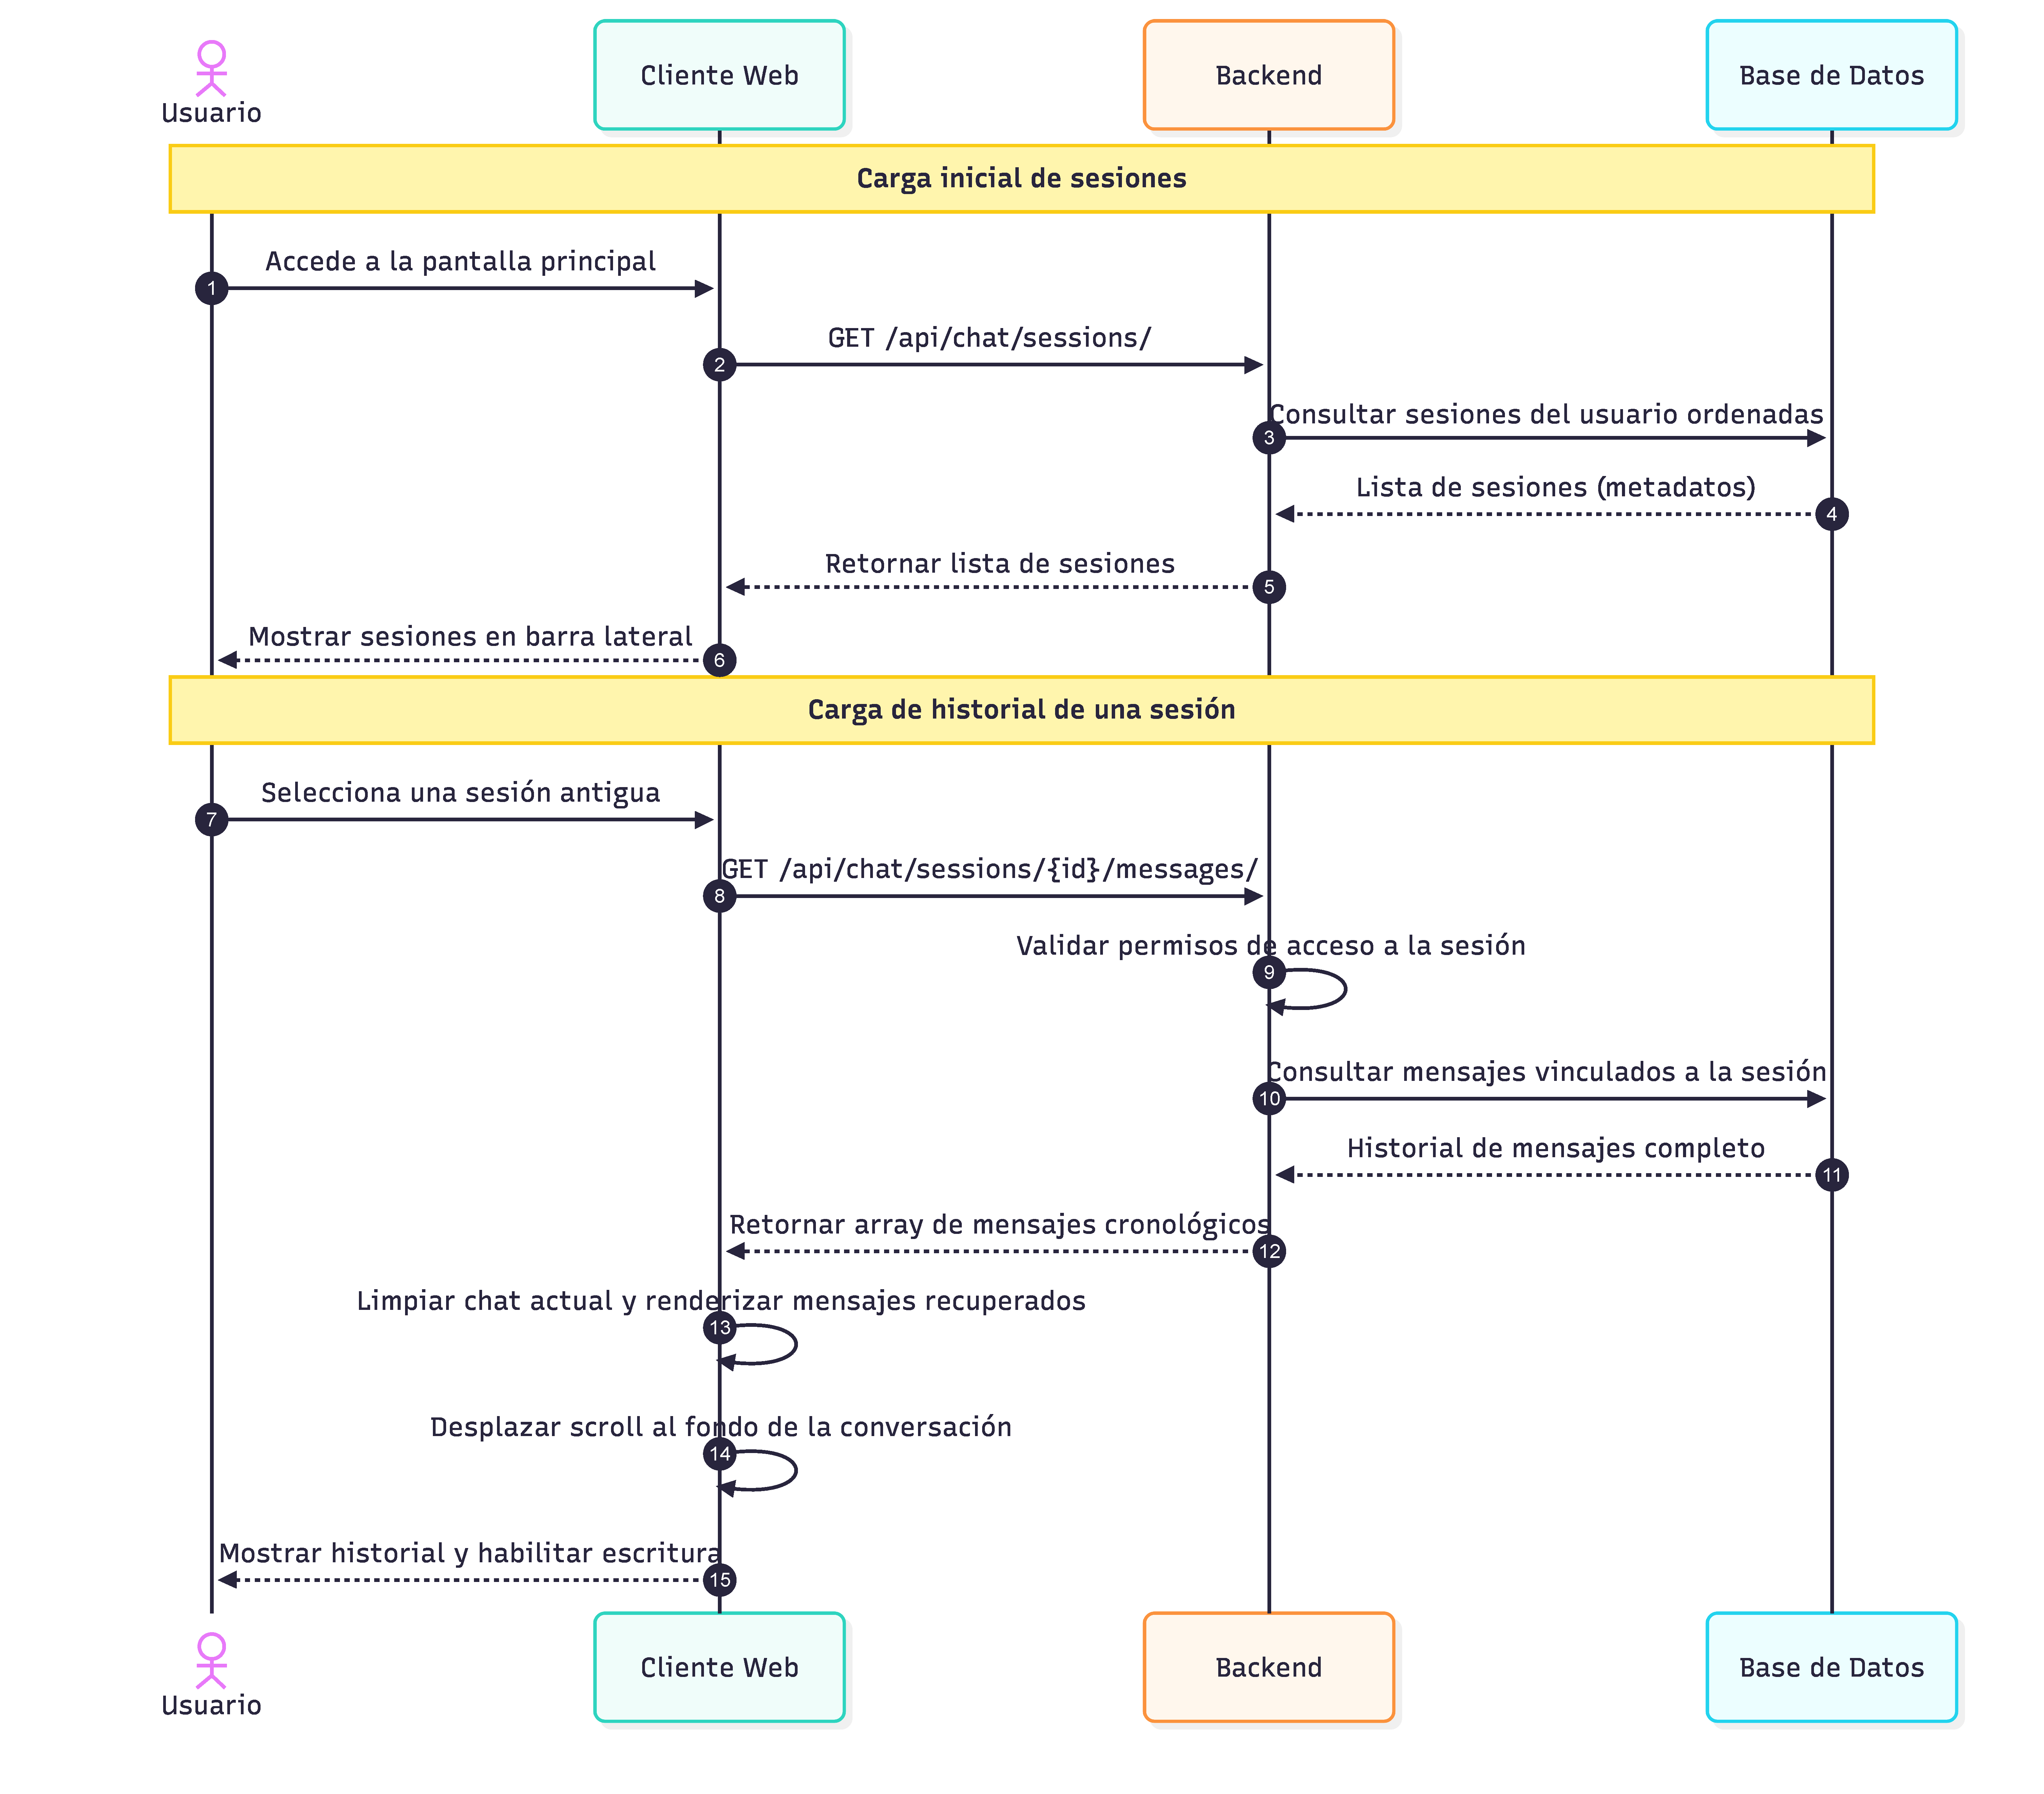
\includegraphics[width=0.85\textwidth]{./diagramas/secuencia_historial_SIMPLE.pdf}
\end{figure}

